\chapter{Implementacja}

W niniejszym rozdziale przedstawiono szczegóły techniczne wdrożonego rozwiązania oraz przybliżono aspekty implementacyjne systemu, obejmujące wykorzystanie platformy Microsoft Power Platform -- w szczególności Power Apps -- do budowy interfejsu użytkownika oraz Power Automate do automatyzacji procesów biznesowych.
Ponadto, omówiono integrację z platformą SharePoint oraz implementację skryptów usprawniających pracę z pakietem Microsoft Office.

W ramach analizy technicznej szczegółowo opisano wszystkie komponenty systemu oraz sposób
ich integracji. Szczególną uwagę poświęcono mechanizmom przepływu danych, automatyzacji procesów oraz implementacji logiki biznesowej w środowisku Low-Code.

\section{Utworzenie bazy danych na platformie Sharepoint}
\sectionauthor{R. Wolniak}

Zgodnie z koncepcją, baza danych utworzona została w środowisku SharePoint.
Pierwszym krokiem jest stworzenie strony dedykowanej temu procesowi. W ekranie startowym programu należy wybrać opcję \emph{Utwórz witrynę}. Następnie należy wybrać typ witryny \emph{Witryna zespołu} oraz szablon określający jej wygląd. Na koniec należy określić nazwę tworzonej strony.

Kolejnym krokiem jest utworzenie struktury list oraz plików. Na potrzeby procesu utworzono dwa foldery -- \emph{TempFiles} przechowujący arkusze przed zapisaniem ich danych na listach oraz \emph{ArchivedFiles} przechowujący pliki po zakończeniu procesu.
Ponadto utworzono trzy listy:
\begin{itemize}
    \item \emph{Lista\_Uslug},
    \item \emph{Lista\_Kwot},
    \item \emph{Lista\_Indykacji}.
\end{itemize}
\hfill \break
Ich struktura jest taka sama jak opisana w podsekcji \ref{Subsec: StrukturaBazyDanych}.
W celu dodania tych elementów należy:
\begin{itemize}
    \item wejść w utworzoną witrynę,
    \item wybrać \emph{Zawartość witryny} z bocznego paska nawigacji,
    \item dodać element przy pomocy przycisku \emph{Nowy},
    \item wybrać typ elementu -- \emph{Biblioteka dokumentów} lub \emph{Lista},
    \item podać nazwę oraz opcjonalnie opis elementu.
\end{itemize}

Po wykonaniu tych kroków, folder jest gotowy do użycia. Jednakże w przypadku list należy jeszcze zdefiniować kolumny. \\Aby to zrobić należy:
\begin{itemize}
    \item wejść w utworzoną listę,
    \item wybrać przycisk \emph{Dodaj kolumnę} znajdujący się po prawej stronie domyślnie utworzonych kolumn,
    \item następnie pojawi się okno z możliwością wyboru typu kolumny oraz jej nazwy,
    \item po zatwierdzeniu podanych opcji, kolumna zostanie dodana do listy.
\end{itemize}

Na koniec należy skonfigurować niektóre kolumny. Aby to zrobić należy wybrać ustawienia strony i nacisnąć pozycję \emph{Ustawienia listy}. Tam wybieramy nazwę kolumny, którą chcemy skofigurować.\\
Tabela \ref{tab:SharepointList} przedstawia konfigurację kolumn listy:
\begin{table}[h]
    \centering
    \caption{Konfiguracja listy na platformie Sharepoint}
    \label{tab:SharepointList}
    \begin{tabular}{|l|l|}
        \hline
        \textbf{Nazwa kolumny}     & \textbf{Typ}             \\ \hline
        Service\_ID                & Liczba                   \\ \hline
        Service\_Name              & Pojedynczy wiersz tekstu \\ \hline
        Service\_Group             & Pojedynczy wiersz tekstu \\ \hline
        Service\_Sub\_Group        & Pojedynczy wiersz tekstu \\ \hline
        Service\_Main\_Group       & Pojedynczy wiersz tekstu \\ \hline
        Instruction\_Link          & Pojedynczy wiersz tekstu \\ \hline
        Unit\_Of\_Measurement      & Pojedynczy wiersz tekstu \\ \hline
        Settlement\_Type           & Pojedynczy wiersz tekstu \\ \hline
        Business\_Service\_Manager & Pojedynczy wiersz tekstu \\ \hline
        Current\_Year\_Plan\_EUR   & Liczba                   \\ \hline
        QTY\_Current\_Year         & Liczba                   \\ \hline
        Next\_Year\_Plan\_EUR      & Liczba                   \\ \hline
        QTY\_Next\_Year            & Liczba                   \\ \hline
        Difference                 & Obliczeniowa             \\ \hline
        MPK                        & Pojedynczy wiersz tekstu \\ \hline
        Year                       & Liczba                   \\ \hline
        IndicationNo               & Liczba                   \\ \hline
        Comment\_Date              & Pojedynczy wiersz tekstu \\ \hline
        Comment\_Author            & Wiele wierszy tekstu     \\ \hline
        Comment\_PZ\_to\_WOB       & Wiele wierszy tekstu     \\ \hline
        Comment\_BSM               & Wiele wierszy tekstu     \\ \hline
        Comment\_K-DES             & Wiele wierszy tekstu     \\ \hline
        Comment\_Intern            & Wiele wierszy tekstu     \\ \hline
        Decision                   & Liczba                   \\ \hline
        Final\_comment             & Wiele wierszy tekstu     \\ \hline
    \end{tabular}
\end{table}

\noindent Kolumna \emph{Difference} jest kolumną obliczeniową co oznacza, że jej wartość jest obliczana względem podanej formuły. W tym przypadku oblicza ona różnicę cen między rokiem następnym a bieżącym. \\
Kolumna \emph{MPK} pomimo wartości liczbowych, jest typu tekstowego gdyż znacznie upraszcza to filtrowanie oraz przepisywanie istniejących numerów do nowych danych. \\
Kolumna \emph{Decision} jest kolumną liczbową ponieważ status decyzji konwertowany jest na kod liczbowy aby przyspieszyć proces filtrowania:
\begin{itemize}
    \item \emph{Accepted} $\rightarrow$ 1,
    \item \emph{Not Accepted} $\rightarrow$ -1,
    \item \emph{No Status} $\rightarrow$ 0.
\end{itemize}




\section{Ekran dodawania danych}
Głównym wyzwaniem okazał się brak systematycznej organizacji danych w arkuszach programu
Excel, co skutkowało niekompatybilnością z zaprojektowaną bazą danych. W celu rozwiązania tego
problemu, opracowano dedykowany interfejs w aplikacji, który wspomaga użytkownika w procesie
przetwarzania danych, minimalizując ryzyko wystąpienia błędów. Składa się on z:
\begin{itemize}
    \item sekcji pozwalającej użytkownikowi na zapisanie pliku w chmurze,
    \item formularza walidacji nazw kolumn,
    \item kontrolek umożliwiających wybór roku i numeru indykacji oraz przycisku do przesłania danych do bazy,
    \item formularza do uzupełniania lub edycji numerów MPK.
\end{itemize}

% \noindent Rysunek \ref{fig:managedatascreen} przedstawia finalny wygląd ekranu dodawania danych do systemu. Komponenty znajdujące się na ekranie zostały opisane poniżej.
% \begin{figure}[H]
%     \centering
%     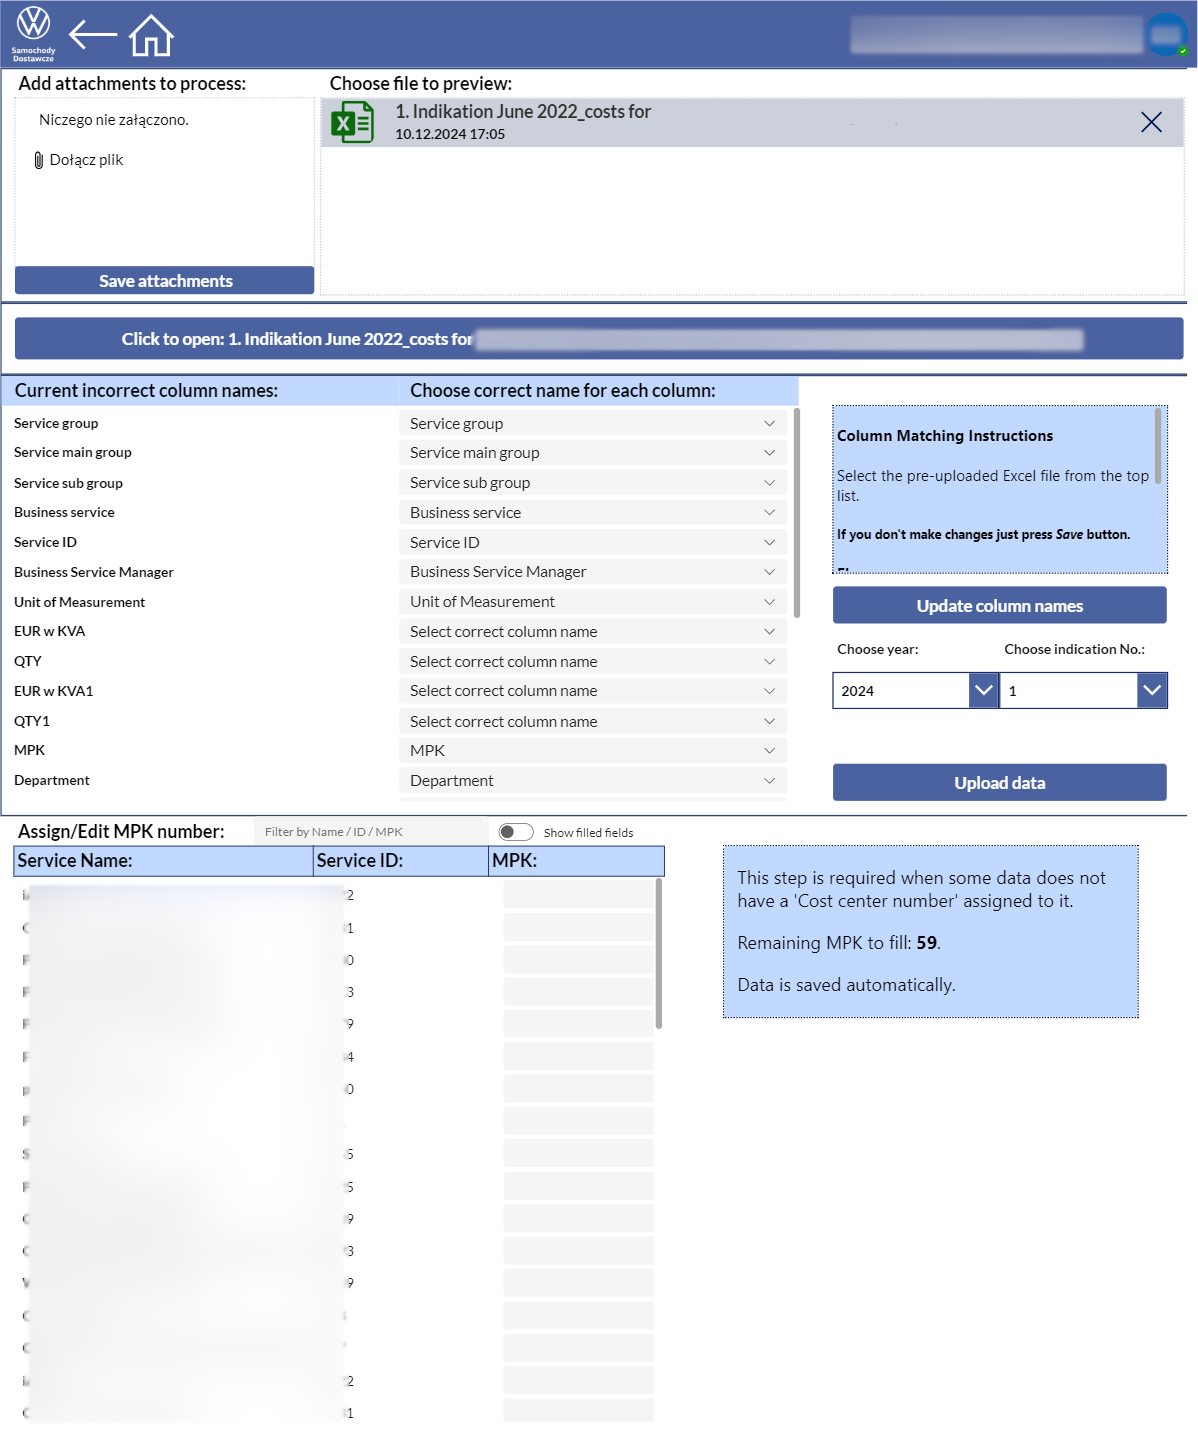
\includegraphics[width=0.9\textwidth]{figures/ManageDataScreen.png}
%     \caption{Ekran dodawania danych do systemu} 
%     \label{fig:managedatascreen}
% \end{figure}

\subsection{Zapis pliku w chmurze}
Pierwszym etapem procesu jest tymczasowy zapis pliku Excel w chmurze, co umożliwia jego udostępnienie innym systemom. Do realizacji tego zadania wykorzystano kontrolkę\footnote{Kontrolka -- element służący do nawigacji, wyświetlania danych i obsługi aplikacji.} \emph{Attachment Control}. Pozwala ona na zapisanie pliku w pamięci aplikacji. Odbywa się to przez naciśnięcie przycisku \emph{"Attach file"} lub przy użyciu mechaniki \emph{przeciągnij i upuść} (\english{Drag And Drop}).

Pod kontrolką \emph{Attachment Control} dodano przycisk \emph{Save attachment}. Jego naciśnięcie skutkuje wywołaniem szeregu funkcji opisanych we właściwości \emph{OnSelect}:
\begin{itemize}
    \item spawdzenie czy plik został poprawnie załadowany,
    \item wywołanie przepływu \emph{SaveFileAndRunScript},
    \item zapisanie wyniku przepływu w zmiennej tablicowej \emph{FlowOutput} (w Power Apps określanej jako \emph{kolekcja}),
    \item po poprawnym zapisaniu pliku w folderze SharePoint, usunięcie go z pamięci aplikacji.
\end{itemize}

% Aby dalej przekazać plik oraz jego zawartość należy nacisnąć przycisk opisany jako \emph{Save attachments} znajdujący się pod wcześniej omawianym elementem. Naciśnięcie go skutkuje wywołaniem szeregu funkcji opisanych we właściwości \emph{OnSelect}. W pierwszej kolejności sprawdzane jest, czy plik został załadowany. Jeśli tak, to wywoływany jest przepływ \emph{SaveFileAndRunScript}. Wynik przepływu jest zapisywany w zmiennej tablicowej, która w Power Apps określana jest jako \definicja{kolekcja}, o nazwie \emph{FlowOutput}. Po wykonaniu się przepływu, pliki zapisane w folderze SharePoint, zostają usunięte z pamięci aplikacji.



\subsubsection*{Przepływ SaveFileAndRunScript}
\label{childflow}
Rysunek \ref{fig:savefileandrunscript}, przedstawia edytor programu Power Automate. Widoczny w nim przepływ nazwany \emph{SaveFileAndRunScript} jest odpowiedzialny za zapisanie pliku w chmurze oraz wstępne przetworzenie. W momencie wywołania przepływu, plik jest przekazany jako parametr wejściowy. Przepływ ten składa się z kilku kroków, które zostaną omówione w kolejności ich wykonywania.

\begin{figure}[t]
    \centering
    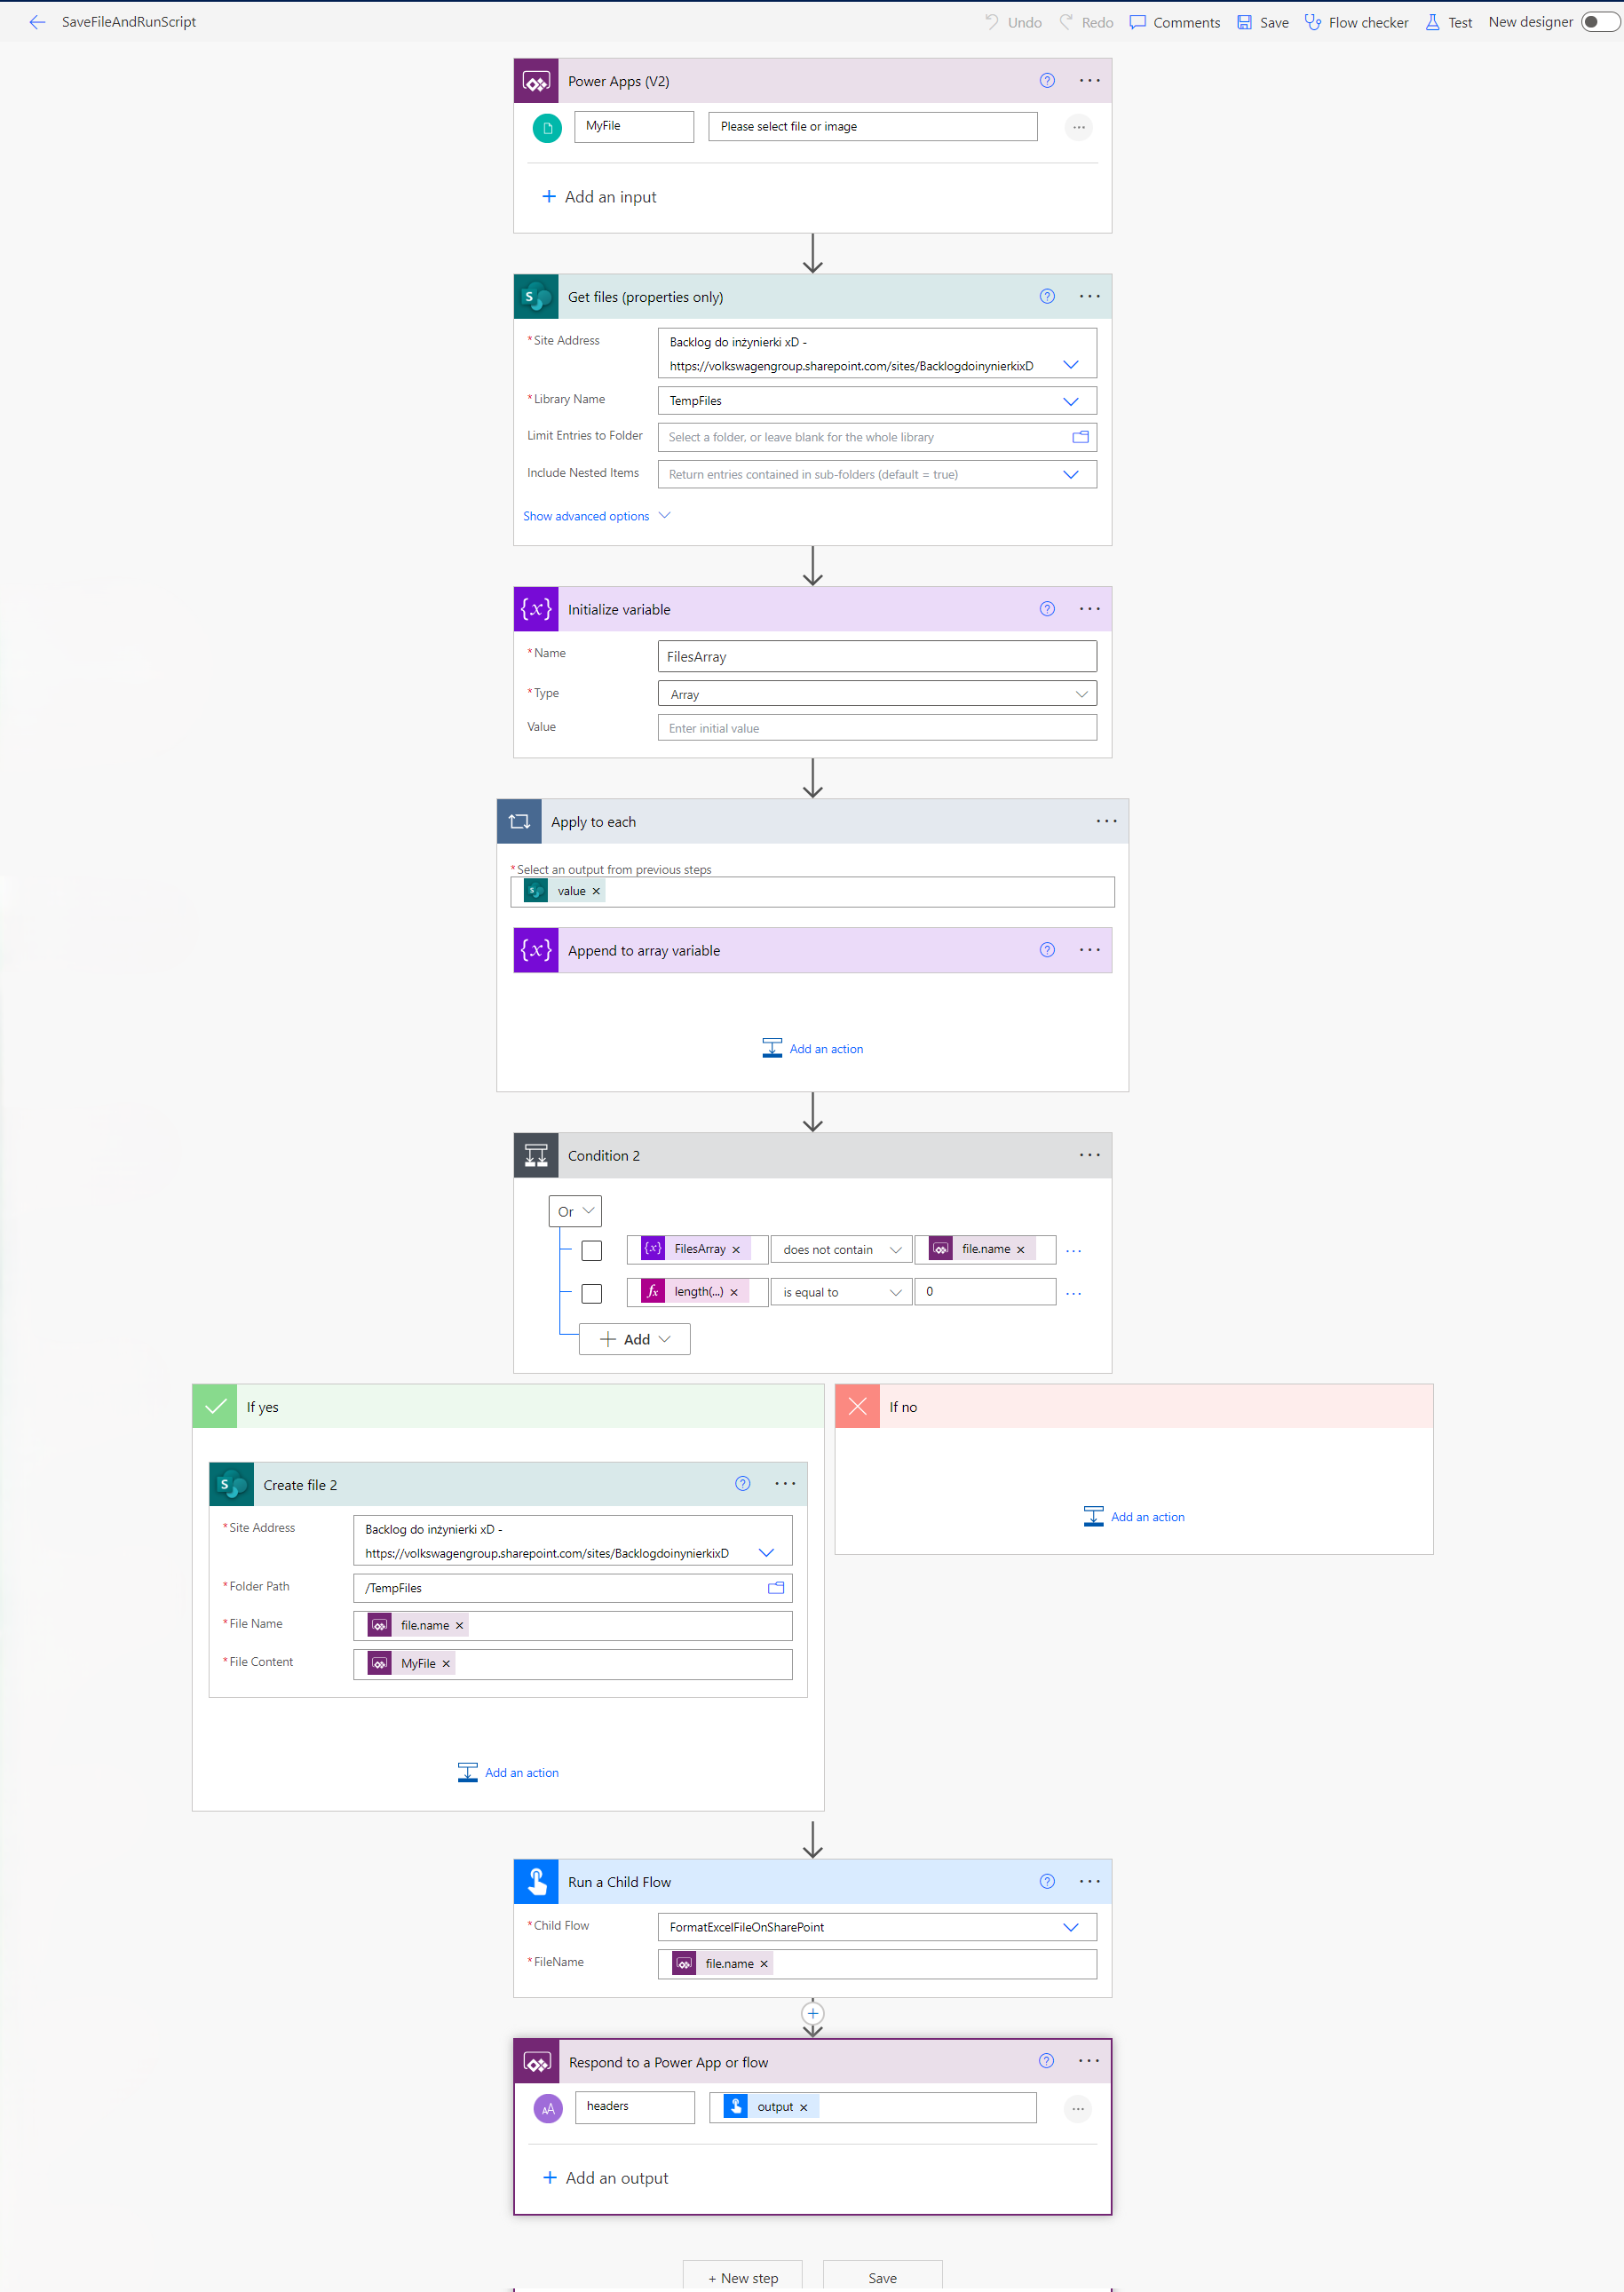
\includegraphics[width=0.9\textwidth]{figures/SaveFileAndRunScript.png}
    \caption{Widok przepływu SaveFileAndRunScript}
    \label{fig:savefileandrunscript}
\end{figure}


\begin{enumerate}
    \item \textbf{Funkcja: Power Apps (V2)} \\
          Przepływ rozpoczyna się od funkcji oczekującej na wywołanie przepływu bezpośrednio z aplikacji Power Apps. Jako parametry wejściowe przyjmuje:
          \begin{itemize}
              \item nazwę pliku (\textit{File Name}),
              \item zawartość pliku (\textit{File Content}) w formacie binarnym.
          \end{itemize}

    \item \textbf{Zainicjowanie zmiennej} \\
          Element \textit{Initialize variable} tworzy zmienną o nazwie \textit{FileExists}, która przechowuje informację, czy plik o podanej nazwie znajduje się już na SharePoint.

    \item \textbf{Sprawdzenie istniejących plików} \\
          Blok \textit{Get files} pobiera listę wszystkich plików z wybranego folderu SharePoint wraz z ich metadanymi, takimi jak nazwa, ścieżka czy data modyfikacji. Wynik zostaje zapisany w zmiennej \textit{FileExists}, która przyjmuje wartość \textit{true}, jeśli plik został znaleziony, lub \textit{false}, jeśli plik nie istnieje.

    \item \textbf{Instrukcja warunkowa \emph{If}} \\
          Element \textit{Condition} sprawdza wartość zmiennej \textit{FileExists}. W zależności od wyniku:
          \begin{itemize}
              \item jeśli zmienna ma wartość \textit{true} -- przepływ kończy działanie,
              \item jeśli zmienna ma wartość \textit{false} -- przepływ kontynuuje proces zapisu.
          \end{itemize}

    \item \textbf{Utworzenie pliku} \\
          Blok \textit{Create file} tworzy nowy plik w SharePoint, wykorzystując parametry:
          \begin{itemize}
              \item adres witryny SharePoint,
              \item ścieżkę do folderu docelowego,
              \item nazwę pliku,
              \item zawartość pliku.
          \end{itemize}

    \item \textbf{Uruchomienie przepływu podrzędnego} \\
          Po pomyślnym zapisaniu pliku przepływ wywołuje tzw. \textit{child flow}, który inicjuje działanie skryptu Office. Skrypt ten odpowiada za przetworzenie pliku w sposób zgodny z założeniami aplikacji. Jego wynik w formacie JSON jest zwracany do strumienia nadrzędnego.

    \item \textbf{Odpowiedź do aplikacji} \\
          Blok \textit{Respond to Power Apps} kończy przepływ, zwracając do aplikacji dane w formacie JSON, przetworzone przez wspomniany skrypt.
\end{enumerate}

\subsection{Skrypt pakietu Office}
Po utworzeniu pliku w SharePoint, w ramach przepływu następuje jego przetworzenie przez skrypt. Jest to niezbędne, jeśli chodzi o działanie procesu. Domyślnie otrzymane dane w pliku Excel są niewidoczne dla większości systemów, mogą one odczytać jedynie informacje zorganizowane w \emph{tabele programu Excel}\footnote{Tabela w programie Excel wymaga osobnej deklaracji poprzez zaznaczenie zakresu komórek i wybór opcji \emph{Narzędzia główne}$\to$\emph{Formatuj jako tabelę}}. Dlatego też powstał skrypt, który działa bezpośrednio w arkuszu. Jego zadaniem jest automatyczne utworzenie tabeli oraz dostosowanie jej do wymagań systemu. Poniżej przedstawiono kroki działania skryptu:

\begin{enumerate}
    \item \textbf{Wybór arkusza roboczego} \\
          Skrypt identyfikuje arkusz zawierający dane, analizuje zakres używanych komórek i usuwa ochronę hasłem, jeśli jest aktywna -- krok ten jest wymagany, aby wprowadzanie zmian w arkuszu było możliwe.

    \item \textbf{Analiza danych} \\
          Skrypt rozpoczyna analizę od wyszukiwania początku tabeli w arkuszu. Następnie:
          \begin{itemize}
              \item usuwa puste kolumny, które nie zawierają żadnych danych,
              \item tworzy tabelę o dynamicznym rozmiarze, uwzględniając zakres danych znajdujących się w arkuszu,
              \item uzupełnia brakujące komórki w kluczowych kolumnach, korzystając z danych w poprzednich wierszach.
          \end{itemize}
          Takie podejście pozwala na uporządkowanie danych i przygotowanie ich do dalszego przetwarzania.

    \item \textbf{Dopasowanie nazw kolumn} \\
          Skrypt porównuje istniejące nazwy kolumn z listą standardowych nagłówków, korzystając z algorytmu \textit{Jaro-Winkler}. Algorytm ten:
          \begin{itemize}
              \item analizuje podobieństwo tekstów, porównując wspólne znaki oraz ich kolejność,
              \item przyznaje dodatkowe punkty za zgodność początkowych znaków (prefiksu),
              \item zwraca wynik jako wartość z przedziału od 0 do 1, gdzie wartości bliższe 1 oznaczają większe podobieństwo.
          \end{itemize}
          Wynik tego procesu jest wykorzystywany w dalszych etapach aplikacji, m.in. do walidacji struktury danych. Jeśli podobieństwo jest mniejsze niż 90\%, skrypt sugeruje ręczne dopasowanie nazwy kolumny.

    \item \textbf{Zwrócenie wyników} \\
          Skrypt generuje JSON zawierający mapowanie oryginalnych nazw kolumn z najlepszymi dopasowaniami z listy standardowych nagłówków.
\end{enumerate}


Kolejnym elementem tej sekcji ekranu jest lista zapisanych plików znajdująca się obok kontrolki \emph{Attach Control}. Umożliwia ona wybór pliku do dalszego przetwarzania. Poniżej umieszczono przycisk \emph{"Click to open:..."}, który pozwala na otwarcie wybranego pliku w nowym oknie przeglądarki przy użyciu funkcji \emph{Launch}. Możliwość podglądu ma na celu ułatwienie weryfikacji jego poprawności.

\subsubsection*{Algorytm Jaro-Winkler}
Podstawą algorytmu, jest algorytm \emph{Jaro}. Polega on na porównaniu dwóch ciągów znaków w celu określenia ich podobieństwa. Wynik obliczany jest na podstawie równania \ref{eq:Jaro}:
\begin{equation}
    \label{eq:Jaro}
    J = \frac{1}{3} \left( \frac{m}{|s_1|} + \frac{m}{|s_2|} + \frac{m - t}{m} \right) \mbox{dla } m>0
\end{equation}
\noindent gdzie:\\
$m$ – liczba dopasowanych znaków,\\    $t$ – liczba transpozycji,\\    $|s_1|$, $|s_2|$ – długości ciągów.\\

\noindent Wynikiem równania, jest wartość z przedziału od 0 do 1, gdzie 1 oznacza pełne dopasowanie. 

Algorytm \emph{Jaro-Winkler} jest rozszerzeniem algorytmu \emph{Jaro}, które dodaje premię za zgodność początkowych znaków. Wynik obliczany jest na podstawie równania \ref{eq:JaroWinkler}:
\begin{equation}
    \label{eq:JaroWinkler}
    JW = J + l \cdot p \cdot (1 - J),
\end{equation}
gdzie:\\
$l$ – długość wspólnego prefiksu (maksymalnie 4 znaki),\\ $p$ – współczynnik skalowania.\\

\noindent Rozszerzona wersja algorytmu, pozwala na bardziej precyzyjne porównanie ciągów znaków, które mają wspólny prefix, co jest szczególnie ważne w przypadku nagłówków kolumn rozpoczynających się od frazy \emph{Service}.


\vspace{1cm}

\textcolor{red}{LINK DO TEGO JARO\_WINKLERA: https://crucialbits.com/blog/a-comprehensive-list-of-similarity-search-algorithms/
https://en.wikipedia.org/wiki/Jaro\%E2\%80\%93Winkler\_distance
}


\subsection{Walidacja nazw kolumn} Kolejnym etapem przed zapisaniem danych do bazy jest walidacja nazw kolumn. W tym celu zaimplementowano formularz zawierający \emph{galerię} -- element umożliwiający wyświetlanie wielu rekordów danych o różnych typach. Pola wyświetlające dane w galerii mogą być dostosowywane w dowolny sposób w zależności od potrzeb użytkownika.

\noindent Galeria składa się z dwóch kolumn:
\begin{itemize}
    \item Lewa kolumna prezentuje obecne nazwy kolumn, które są wyświetlane za pomocą kontrolki \emph{Label}\footnote{\emph{Label} -- kontrolka tekstowa umożliwiająca wyświetlanie statycznych wartości.}.
    \item Prawa kolumna zawiera kontrolkę \emph{ComboBox}\footnote{\emph{ComboBox} -- rozwijana lista z możliwością wprowadzania tekstu}, która umożliwia wybór nazwy ze standardowej listy nagłówków. Wartości domyślne, widoczne w kontrolkach \emph{ComboBox}, są generowane przez wcześniej opisany skrypt w taki sposób, aby do oryginalnej nazwy kolumny dopasowana została najbardziej podobna nazwa z predefiniowanej listy nagłówków. Ma to na celu minimalizację danych wprowadzonych przez użytkownika.
\end{itemize}

Po prawej stronie formularza umieszczono instrukcję użytkownika, zawierająca wskazówki dotyczące prawidłowego uzupełniania nazw kolumn. Poniżej instrukcji dodano przycisk \emph{Update column names}, który umożliwia zapisanie zmian w strukturze danych.

\noindent Działanie tego mechanizmu opiera się na zastosowaniu skryptu pakietu Office, wywoływanego przy użyciu kolejnego przepływu. Skrypt jako parametr wejściowy przyjmuje zmienną tablicową w formacie JSON, zawierającą mapowanie oryginalnych nazw kolumn z poprawionymi wartościami wybranymi przez użytkownika. Następnie skrypt iteruje po wierszu zawierającym nagłówki kolumn i dokonuje ich zamiany zgodnie z otrzymaną mapą. Po zakończeniu działania skrypt zwraca nową strukturę nazw kolumn.

Pod przyciskiem \emph{Update column names} umieszczone zostały kontrolki \emph{Dropdown}\footnote{\emph{Dropdown} -- kontrolka umożliwiająca wybór jednej z dostępnych wartości z rozwijanej listy, bez możliwości edycji.} oraz przycisk \emph{Upload data}, które są kluczowe dla kolejnego etapu przetwarzania danych, obejmującego ich integrację z listami SharePoint.


% \begin{figure}[t]
%     \centering
%     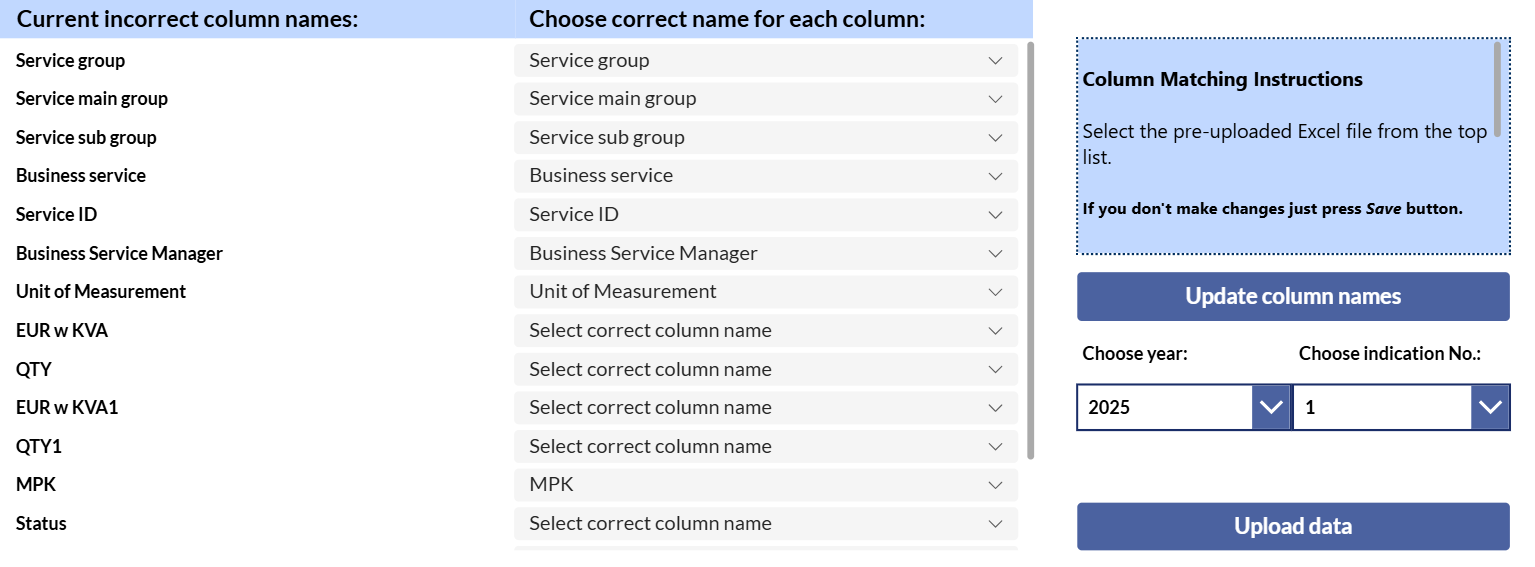
\includegraphics[width=\textwidth]{figures/ColumnMappingForm.png}
%     \caption{Formularz walidacji nazw kolumn}
%     \label{fig:columnmappingform}
% \end{figure}

\subsection{Integracja z listami SharePoint} Po zakończeniu walidacji nazw kolumn, kolejnym etapem jest zapisanie przetworzonych danych w utworzonej strukturze SharePoint. Proces ten rozpoczyna się od wyboru roku i numeru indykacji przy użyciu dedykowanych kontrolek \emph{Dropdown}. Wybrane wartości są następnie wykorzystywane podczas importu danych do odpowiednich list, co odbywa się za pomocą przycisku \emph{Upload data}.

Skutki kliknięcia przycisku mogą się różnić w zależności od wybranych wartości i tego czy nazwy kolumny zostały zmienione. Jeśli przed próbą wgrania danych, nie został wciśnięty przycisk \emph{Update column names}, system wyświetla okno z zapytaniem o poprawność nazw kolumn w celu upewnienia się, że użytkownik nie wgra przypadkowo danych z niepoprawnymi nagłówkami.
Kiedy jednak nazwy kolumn zostały zmienione, ale użytkownik wybrał rok oraz numer indykacji, istniejące w bazie danych, system wyświetla zapytanie czy użytkownik chce nadpisać dane, które już tam się znajdują czy też anulować operacje. W momencie kiedy nazwy kolumn nie zostaną zmienione oraz dane z wybranym rokiem i numerem indykacji istnieją w bazie danych, pojawiają się oba okna z informacjami.


% Rysunki \ref{fig:CorrectHeadersPopup} oraz \ref{fig:DoYouWantToOverwrite} przedstawiają dwa możliwe scenariusze, które mogą wystąpić po naciśnięciu przycisku.
% \begin{figure}[htbp]
%     \centering
%     % Pierwszy obrazek
%     \begin{minipage}{0.48\textwidth}
%         \centering
%         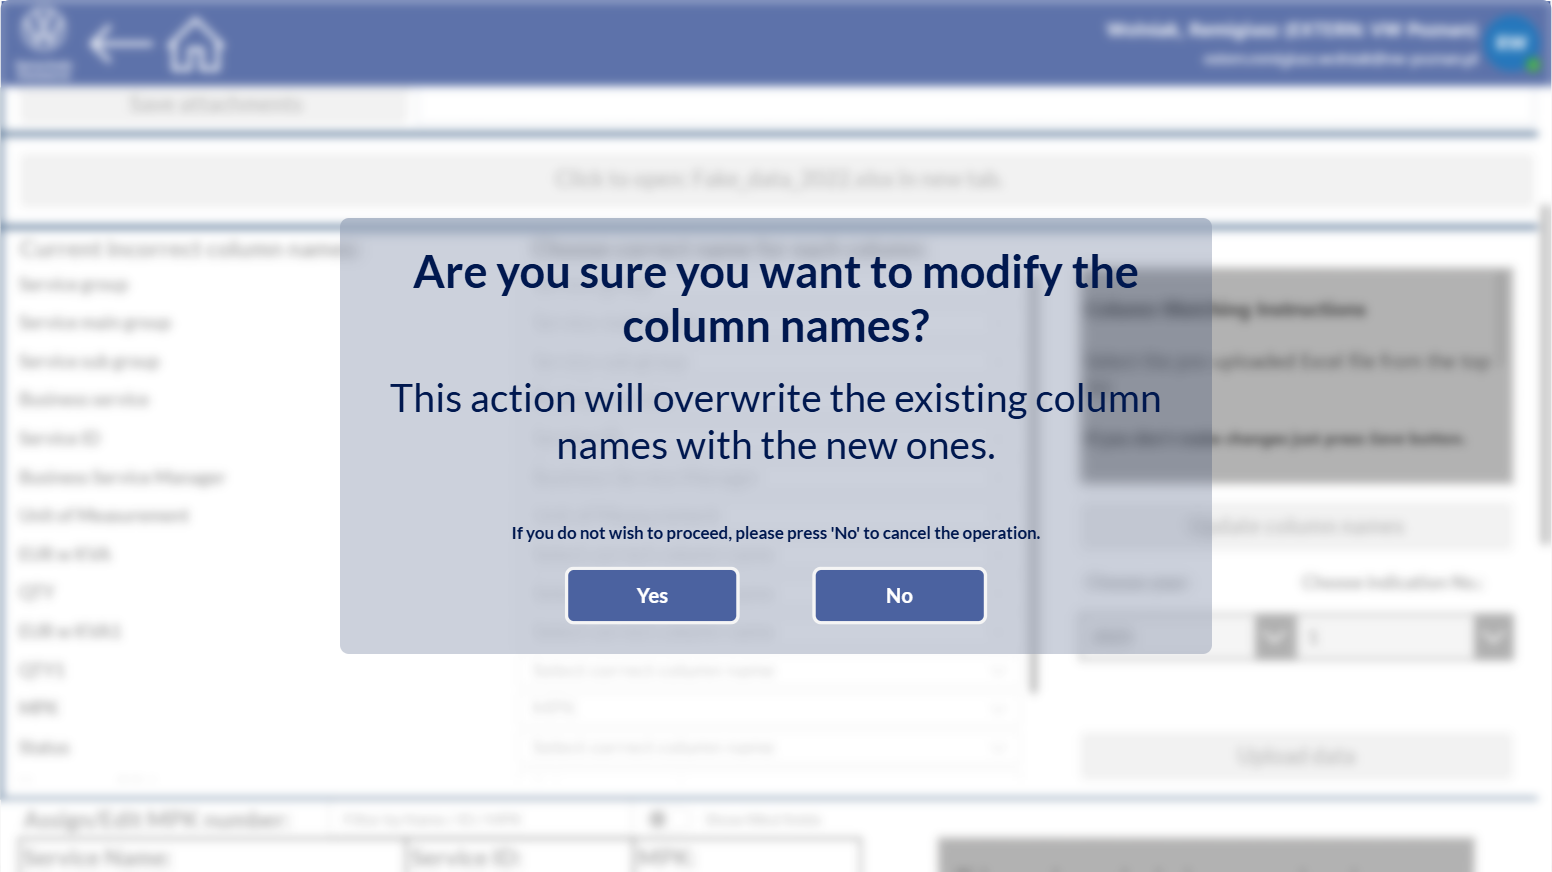
\includegraphics[width=\linewidth]{figures/CorrectHeadersPopup.png}
%         \caption{Zapytanie o poprawność nazw kolumn}
%         \label{fig:CorrectHeadersPopup}
%     \end{minipage}\hfill
%     % Drugi obrazek
%     \begin{minipage}{0.48\textwidth}
%         \centering
%         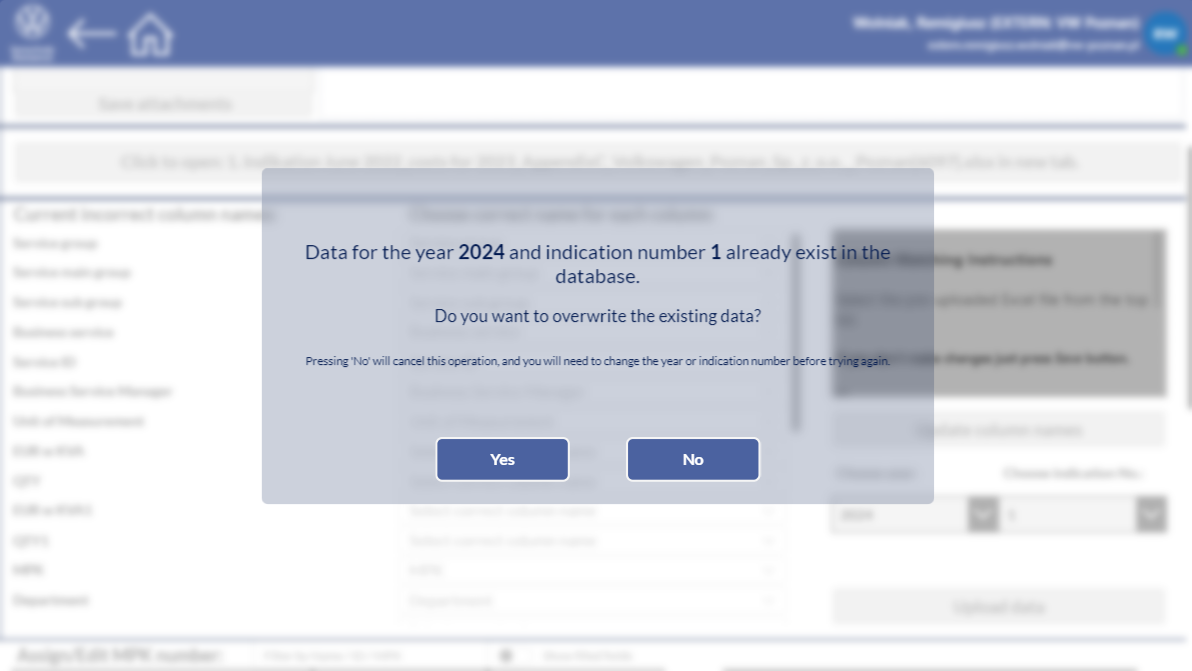
\includegraphics[width=\linewidth]{figures/DoUWantToOverwrite.png}
%         \caption{Zapytanie o nadpisanie danych}
%         \label{fig:DoYouWantToOverwrite}
%     \end{minipage}
%     \label{fig:obrazki}
% \end{figure}

Kiedy użytkownik upewni się, że wszystkie dane są poprawne i zatwierdzi operację, system przystępuje do importu danych. W tym celu wywołuje kolejny przepływ w programie Power Automate, który przypisuje informacji do odpowiednich list w bazie danych upewniając się jednocześnie, że nie zostaną dodane duplikaty rekordów.

\noindent Przepływ ten jest bardzo rozbudowany, dlatego zamiast widoku edytora Power Automate, na rysunku \ref{fig:flowchart} pokazany został schemat blokowy, który reprezentuje kolejność wykonywania poszczególnych kroków. Został on uproszczony, ponieważ bloku umieszczone w błękitnych ramkach, powinny być powielone do trzech równoległych gałęzi. Wynika to z faktu, że dla wszystkich list procedura jest identyczna, a różnicą są m.in. nazwy list użyte strukturze żądań HTTP. Ponadto elementy, które mają przerywaną, pomarańczową ramkę to elementy, które znajdują się w głęzi dotyczącej listy kwot. Odpowiadają one za pobieranie i przepisywanie numeru MPK z roku wcześniej.


% Zmodyfikowane style z dodaną czcionką \large
\tikzstyle{startstop} = [rectangle, rounded corners, minimum width=3cm, minimum height=1cm, text centered, line width=2pt, draw={rgb,255:red,116; green,39; blue,116}, fill={rgb,255:red,234; green,223; blue,234}]

\tikzstyle{processExcel} = [rectangle, minimum width=3cm, minimum height=1cm, text centered, line width=2pt, draw={rgb,255:red,16; green,124; blue,65}, fill=ForestGreen!80]

\tikzstyle{Variable} = [rectangle, minimum width=3cm, minimum height=1cm, text centered, line width=2pt, draw={rgb,255:red,119; green,11; blue,214}, fill={rgb,255:red,171; green,104; blue,230}]

\tikzstyle{Data} = [rectangle, minimum width=3cm, minimum height=1cm, text centered, line width=2pt, draw={rgb,255:red,140; green,108; blue,255}, fill={rgb,255:red,166; green,141; blue,255}]

\tikzstyle{SP} = [rectangle, minimum width=3cm, minimum height=1cm, text centered, line width=2pt, draw={rgb,255:red,3 ; green,108; blue,112}, fill={rgb,255:red,39; green,181; blue,194}, align=center]

\tikzstyle{decision} = [diamond, minimum width=3cm, minimum height=1cm, text centered, draw=black, fill=green!30]

\tikzstyle{decision} = [diamond, minimum width=3cm, minimum height=1cm, text centered, draw=black, fill=green!30]
\tikzstyle{arrow} = [thick,->,>=stealth]
\tikzstyle{data} = [parallelogram, minimum width=3cm, minimum height=1cm, text centered, draw=black, fill=yellow!30]
\begin{figure}
    \resizebox{0.95\textwidth}{!}{%
        
\begin{tikzpicture}[node distance=3cm]
   
% Start node
\node (start) [startstop, text width=8cm, align=center] {\textbf{Trigger: Power Apps} \\[4pt]
\begin{tabular}{@{}cc@{}}
    FileName (string) & Year (number) \\
    IndicationNo (number) & Overwrite (bool) \\
\end{tabular}};

% Process nodes
\node (getTables) [processExcel, below of=start, fill=ForestGreen!80, text width=6cm, align=center, yshift=0.5cm] {\textbf{Get Tables} \\[4pt]
(from Excel with name \textit{FileName})};

\node (initializeVars) [Variable, align=center, text width=12cm, below of=getTables, yshift=-0.5cm] {
\textbf{Initialize Variables:}\\[4pt]
\begin{tabular}{@{}ll@{}}
- ExcelFile (Array) & - ItemsAddedToListaUslug (String) \\
- ItemsAddedToListaKwot (String) & - ItemsAddedToListaIndykacji (String) \\
- BatchRequestHeader (String) & - EndOfBatchRequest (String) \\
- Errors (String) \\
\end{tabular}
};


% Loop
% Twój niestandardowy bloczek jako węzeł
\node (applyToEach) [draw=none, inner sep=0pt, below of=initializeVars, below of=initializeVars, yshift=1.5cm] {%
    \begin{tikzpicture}[baseline]
        \draw [fill={rgb,255:red,152; green,171; blue,193}, draw={rgb,255:red,72; green,105; blue,145}, line width=2pt, dashed] (0,0) rectangle (5.5,-3.5);
        \draw [Variable, text width=4.5cm] (0.25,-1.5) rectangle node {\normalsize \textbf{Set Variable} \\[4pt]
        ExcelFile = TableContent} (5.25,-2.75);
        \node [font=\normalsize] at (2.75,-0.5) {\textbf{Apply to each}};
        \draw [processExcel] (0.25,-0.75) rectangle node {\normalsize \textbf{List rows present in table}} (5.25,-1.5);
    \end{tikzpicture}
};

% Select Columns
\node (selectCols) [Data, below of=applyToEach, text width=6cm, align=center] {\textbf{Select Columns from Excel}};

\node (Condition1) [rectangle, minimum width=3cm, minimum height=1cm, text centered, line width=2pt, draw={rgb,255:red,72; green,79; blue,88}, fill={rgb,255:red,149; green,153; blue,158},below of=selectCols, yshift=1cm, text width = 4cm] {\textbf{Condition 1}\\[4pt] \textit{Overwrite} == false};

\coordinate (belowCondition1) at ($(Condition1.south) - (0,2cm)$);


\node (ComplexNode) [draw=none, inner sep=0pt, anchor=north] at (Condition1.south) {%
    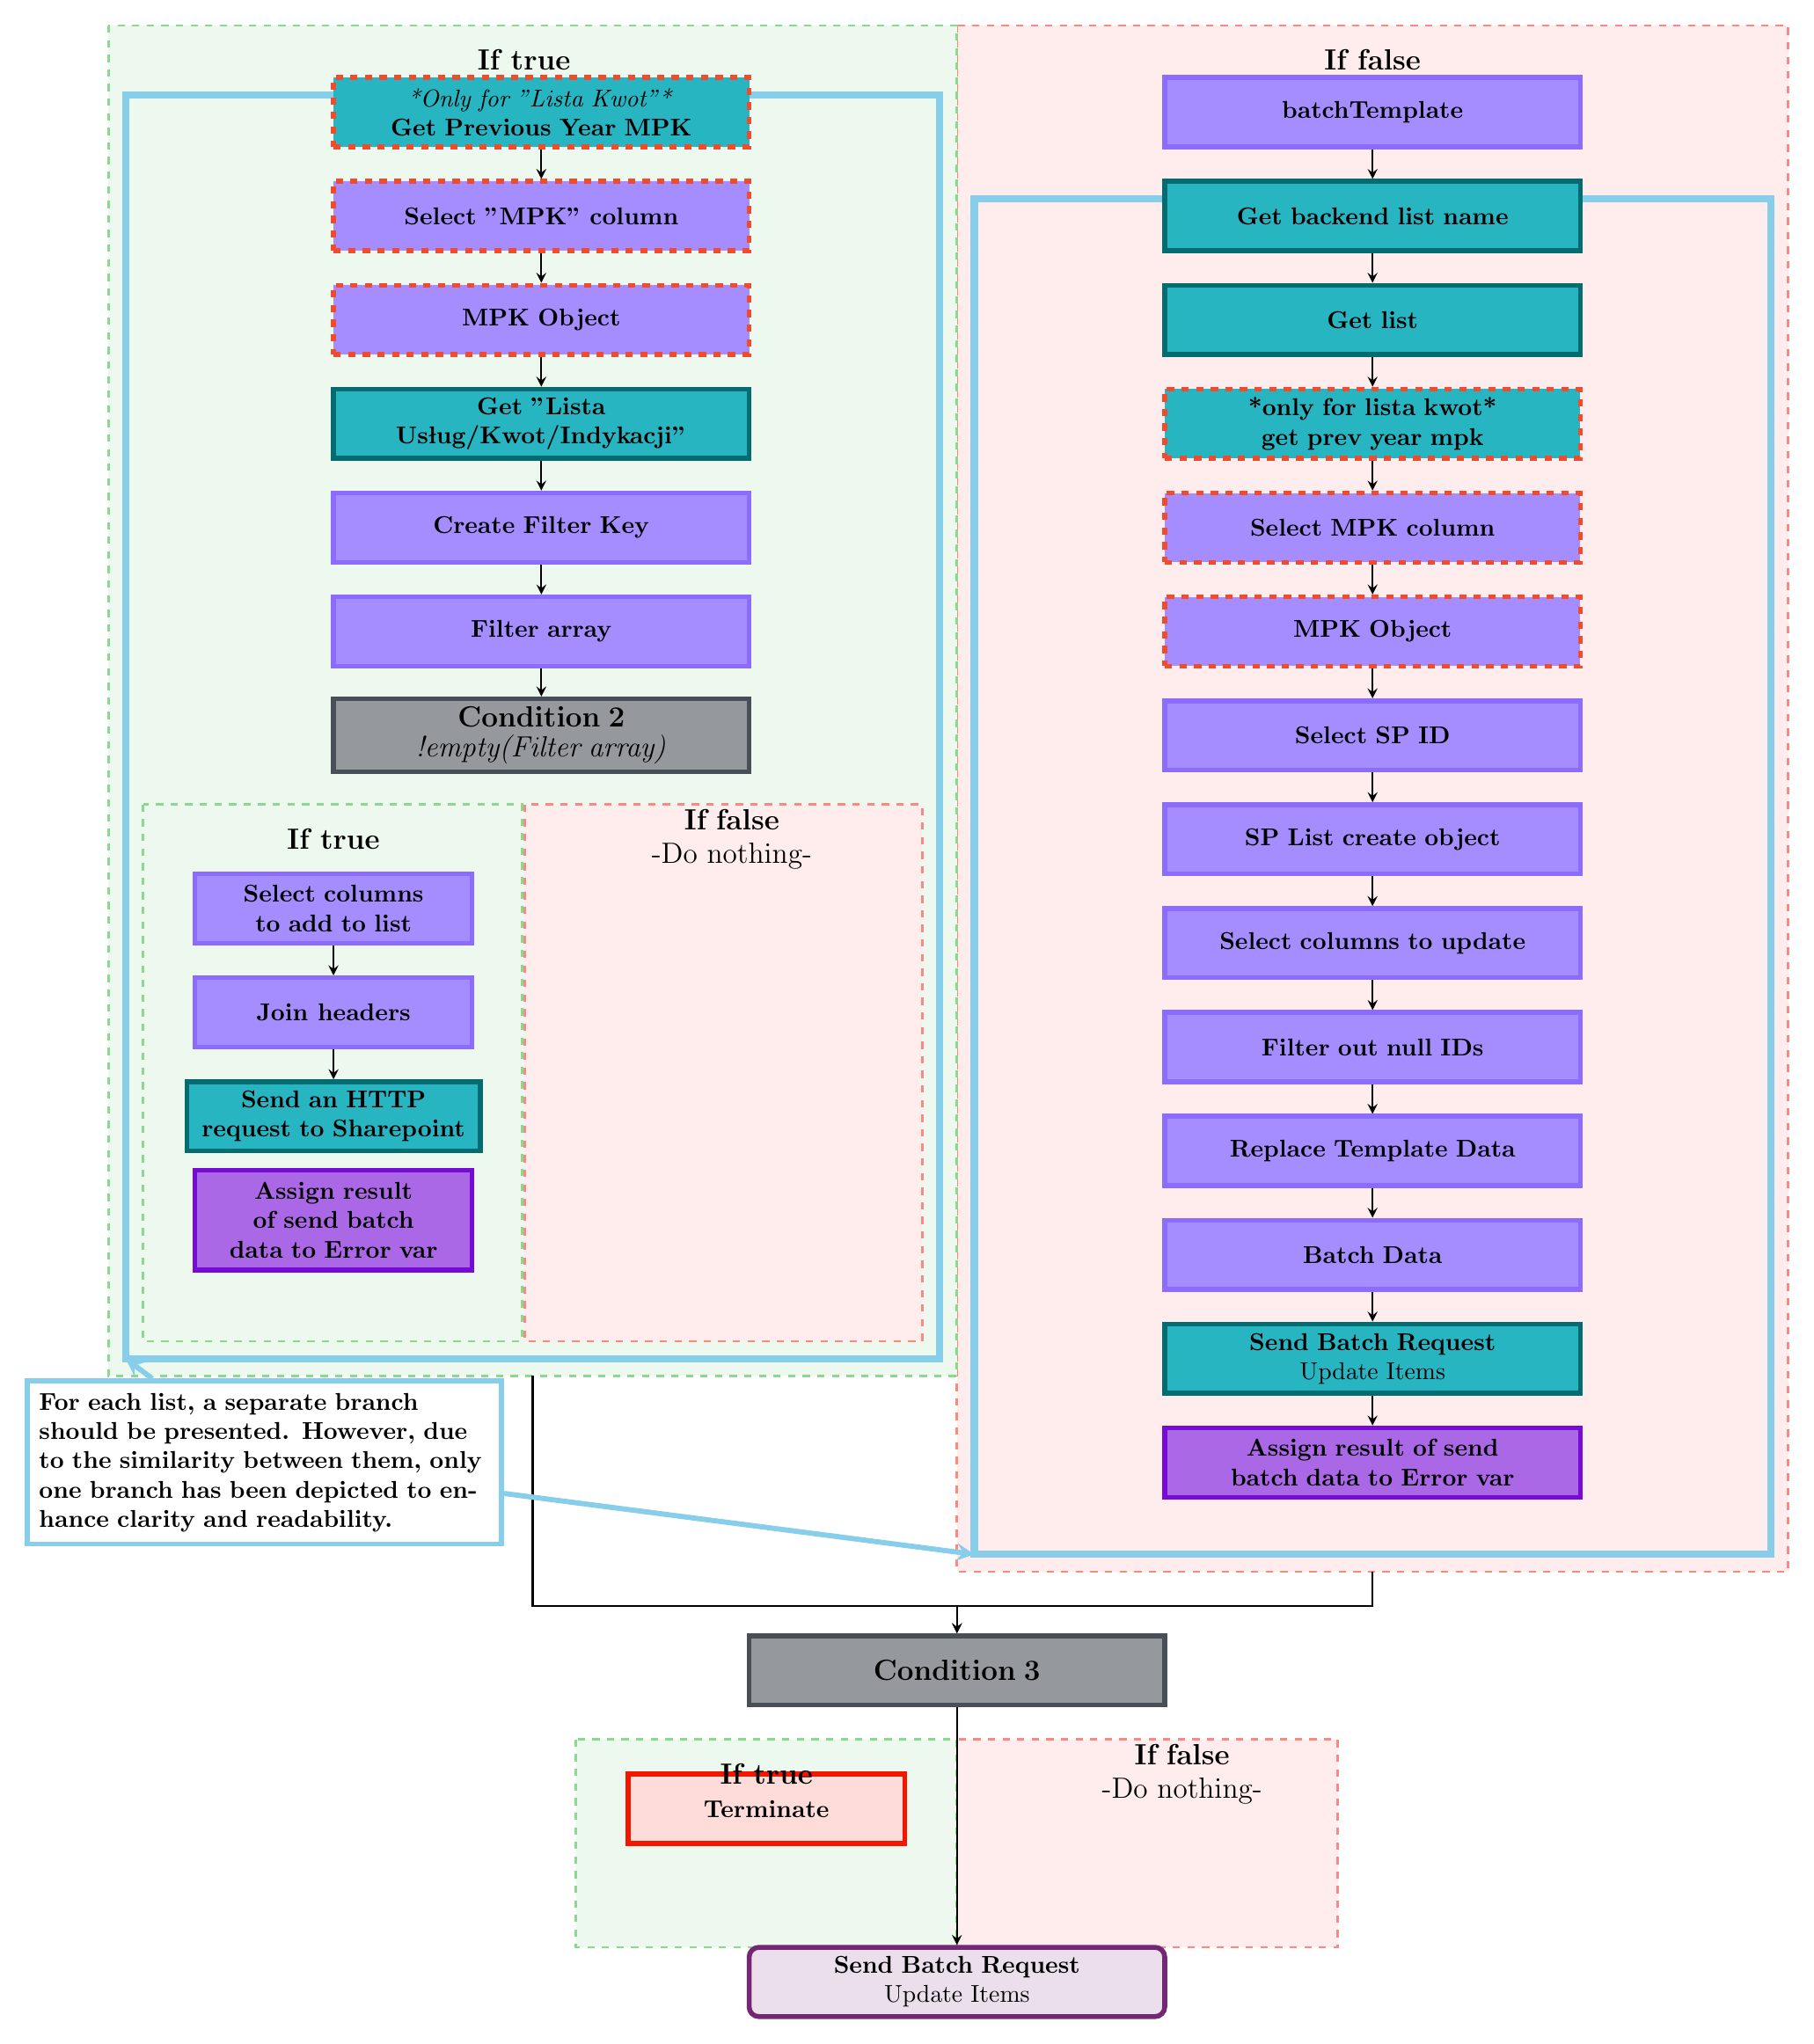
\begin{tikzpicture}[baseline]
\draw [ color={rgb,255:red,251; green,137; blue,129} , fill={rgb,255:red,254; green,237; blue,236}, line width=1pt , dashed] (2,23.75) rectangle  node {}  (14,1.425); %false
\draw [ color={rgb,255:red,136; green,218; blue,141} , fill={rgb,255:red,237; green,249; blue,238}, line width=1pt , dashed] (-10.25,23.75) rectangle  node {}  (2,4.25); %true
\draw [ color=SkyBlue, line width=3pt] (2.25,21.25) rectangle  node {}  (13.75,1.675); %false
\draw [ color=SkyBlue, line width=3pt] (-10,22.75) rectangle  node {}  (1.75,4.5); %true

\node (true1) [SP, dashed, minimum width=6cm, text width=5cm, draw=RedOrange] at (-4,22.5) {\normalsize \emph{*Only for "Lista Kwot"*}\\ \textbf{Get Previous Year MPK}};
\node (true2) [Data, minimum width=6cm, text width=5cm,dashed, draw=RedOrange] at (-4,21) {\normalsize \textbf{Select "MPK" column}};
\node (true3) [Data, minimum width=6cm, text width=5cm,dashed, draw=RedOrange] at (-4,19.5) {\normalsize \textbf{MPK Object}};
\node (true4) [SP, minimum width=6cm, text width=5cm, text width=5cm] at (-4,18) {\normalsize \textbf{Get "Lista Usług/Kwot/Indykacji"}};
\node (true5) [Data, minimum width=6cm, text width=5cm] at (-4,16.5) {\normalsize \textbf{Create Filter Key}};
\node (true6) [Data, minimum width=6cm, text width=5cm] at (-4,15) {\normalsize \textbf{Filter array}};

\draw [ color={rgb,255:red,136; green,218; blue,141} , fill={rgb,255:red,237; green,249; blue,238}, line width=1pt , dashed] (-9.75,12.5) rectangle  node {}  (-4.28,4.75);
\node (true11) [Data, minimum width=4cm, text width=3cm] at (-7,11) {\normalsize \textbf{Select columns to add to list}};
\node (true12) [Data, minimum width=4cm] at (-7,9.5) {\normalsize \textbf{Join headers}};
\node (true13) [SP, minimum width=4cm, text width=4cm] at (-7,8) {\normalsize \textbf{Send an HTTP request to Sharepoint}};
\node (true14) [Variable, minimum width=4cm, text width=3.5cm, inner sep=5pt] at (-7,6.5) { \textbf{Assign result of send batch data to Error var}};
\draw [ color={rgb,255:red,251; green,137; blue,129} , fill={rgb,255:red,254; green,237; blue,236}, line width=1pt , dashed] (-4.24,12.5) rectangle  node {}  (1.5,4.75);
\node (Condition2) [rectangle, minimum width=3cm, minimum height=1cm, text centered, line width=2pt, draw={rgb,255:red,72; green,79; blue,88}, fill={rgb,255:red,149; green,153; blue,158}, minimum width=6cm, text width=5cm] at (-4,13.5) {\large \textbf{Condition 2}\\ \emph{!empty(Filter array)}};
\node [font=\large] at (-4.25,23.25) {\textbf{If true}};
\node [font=\large] at (8,23.25) {\textbf{If false}};
\node [font=\large] at (-7,12) {\textbf{If true}};
\node [font=\large, text width=4cm, align=center] at (-1.25,12) {\textbf{If false}\\-Do nothing-};



\node (false1) [Data, minimum width=6cm, text width=5cm] at (8,22.5) { \textbf{batchTemplate}};
\node (false2) [SP, minimum width=6cm, text width=5cm] at (8,21) { \textbf{Get backend list name}};
\node (false3) [SP, minimum width=6cm, text width=5cm] at (8,19.5) { \textbf{Get list}};
\node (false4) [SP, minimum width=6cm, text width=5cm,dashed, draw=RedOrange] at (8,18) { \textbf{*only for lista kwot* \\ get prev year mpk}};
\node (false5) [Data, minimum width=6cm, text width=5cm,dashed, draw=RedOrange] at (8,16.5) { \textbf{Select MPK column}};
\node (false6) [Data, minimum width=6cm, text width=5cm,dashed, draw=RedOrange] at (8,15) { \textbf{MPK Object}};
\node (false7) [Data, minimum width=6cm, text width=5cm] at (8,13.5) {\textbf{Select SP ID}};
\node (false8) [Data, minimum width=6cm, text width=5cm] at (8,12) { \textbf{SP List create object}};
\node (false9) [Data, minimum width=6cm, text width=5cm] at (8,10.5) { \textbf{Select columns to update}};
\node (false10) [Data, minimum width=6cm, text width=5cm] at (8,9) { \textbf{Filter out null IDs}};
\node (false11) [Data, minimum width=6cm, text width=5cm] at (8,7.5) { \textbf{Replace Template Data}};
\node (false12) [Data, minimum width=6cm, text width=5cm] at (8,6) { \textbf{Batch Data}};
\node (false13) [SP, minimum width=6cm, text width=5cm] at (8,4.5) { \textbf{Send Batch Request}\\ Update Items};
\node (false14) [Variable, minimum width=6cm, text width=5cm] at (8,3) { \textbf{Assign result of send batch data to Error var}};

\draw [ color={rgb,255:red,251; green,137; blue,129} , fill={rgb,255:red,254; green,237; blue,236}, line width=1pt , dashed] (2,-1) rectangle  node {}  (7.5,-4);
\draw [ color={rgb,255:red,136; green,218; blue,141} , fill={rgb,255:red,237; green,249; blue,238}, line width=1pt , dashed] (-3.5,-1) rectangle  node {}  (2,-4);
\node[Data, minimum width=4cm, draw={rgb,255:red,244; green,23; blue,0} , fill={rgb,255:red,253; green,220; blue,217}] at (-0.75,-2) {\normalsize \textbf{Terminate}};
\node (Condition3) [rectangle, minimum width=3cm, minimum height=1cm, text centered, line width=2pt, draw={rgb,255:red,72; green,79; blue,88}, fill={rgb,255:red,149; green,153; blue,158}, minimum width=6cm, text width=5cm] at (2,0) {\large \textbf{Condition 3}};
    \node [font=\large] at (-0.75,-1.5) {\textbf{If true}};
\node [font=\large, text width=4cm, align=center] at (5.25,-1.5) {\textbf{If false}\\-Do nothing-};

\node (stop) [startstop, minimum width=6cm, text width=5cm] at (2,-4.5) { \textbf{Send Batch Request}\\ Update Items};
\node (annotation) [rectangle,text width=6.5cm, draw=SkyBlue,line width=0.75mm, inner sep=5pt] at (-8,3) {\textbf{For each list, a separate branch should be presented. However, due to the similarity between them, only one branch has been depicted to enhance clarity and readability.
}};
%Arrows
\draw [arrow] (true1) -- (true2);
\draw [arrow] (true2) -- (true3);
\draw [arrow] (true3) -- (true4);
\draw [arrow] (true4) -- (true5);
\draw [arrow] (true5) -- (true6);
\draw [arrow] (true6) -- (Condition2);

\draw [arrow] (true11) -- (true12);
\draw [arrow] (true12) -- (true13);

\draw [arrow] (false1) -- (false2);
\draw [arrow] (false2) -- (false3);
\draw [arrow] (false3) -- (false4);
\draw [arrow] (false4) -- (false5);
\draw [arrow] (false5) -- (false6);
\draw [arrow] (false6) -- (false7);
\draw [arrow] (false7) -- (false8);
\draw [arrow] (false8) -- (false9);
\draw [arrow] (false9) -- (false10);
\draw [arrow] (false10) -- (false11);
\draw [arrow] (false11) -- (false12);
\draw [arrow] (false12) -- (false13);
\draw [arrow] (false13) -- (false14);
\draw [arrow] (Condition3) -- (stop);



\draw [arrow] (-4.125,4.25) -- +(0,-3.325) -- +(6.125,-3.325) --(Condition3);
\draw [arrow] (8,1.425) -- +(0,-0.5) -- +(-6,-0.5) --(Condition3);
\draw [arrow, line width=0.75mm, SkyBlue] (annotation) -- (-10,4.5);
\draw [arrow, line width=0.75mm, SkyBlue] (annotation) -- (2.25,1.675);
\end{tikzpicture}

};
\draw [arrow] (start) -- (getTables);
\draw [arrow] (getTables) -- (initializeVars);
\draw [arrow] (initializeVars) -- (applyToEach);
\draw [arrow] (applyToEach) -- (selectCols);
\draw [arrow] (selectCols) -- (Condition1);




\end{tikzpicture}

    }
    \caption{Schemat blokowy procesu importu danych z arkusza kalkulacyjnego do bazy danych}
    \label{fig:flowchart}
\end{figure}

\pagebreak
Poniżej wyjaśniono działanie poszczególnych bloków znajdujących się na schemacie. Elementy oznaczone symbolem (\textasteriskcentered) odnoszą się do bloków znajdujących się w pomarańczowej, przerywanej ramce.
\begin{enumerate}
    \item Blok \textbf{Trigger: Power Apps} jest wyzwalaczem działania przepływu. Uruchamia się kiedy użytkownik wciśnie przycisk w aplikacji. Jako parametry wejściowe przyjmuje nazwę pliku, rok i numer indykacji jakie mają być przypsiane do danych oraz informacje czy nadpisać istniejące rekordy czy też nie.

    \item \textbf{Get Tables} pobiera nazwy wszystkich tabel z pliku o nazwie przekazanej do wyzwalacza (każdy plik powinien zawierać jedną tabelę, ale w Power Automate trzeba pobrać wszystkie możliwe).
    \item Funkcja \textbf{Initialize variable} tworzy następujące zmienne:
          \begin{itemize}
              \item \emph{ExcelFile} -- zmienna tablicowa, przechowująca dane z arkusza,
              \item \emph{ItemsAddedToListaUsług/Kwot/Indykacji} -- te zmienne przechowują \emph{ciało żądania HTTP}, które jest konstruowane w trakcie działania przepływu.
              \item \emph{BatchRequestHeader} oraz \emph{EndOfBatchRequest} -- przechowują one stałe nagłówki i stopkę żądania HTTP, które są wspólne dla wszystkich zapytań.
          \end{itemize}
    \item Pętla \textbf{Apply to each}, dodana automatycznie przez Power Automate, iteruje po nazwach tabel pobranych z pliku a następnie dla każdej z nich przepisuje dane do zmiennej \emph{ExcelFile}.
    \item Funkcja \textbf{Select Columns from Excel}, pozwala na kształtowanie danych. Jako wejście przyjmuje ona dane z \emph{ExcelFile} a następnie mapuje wartości tej zmiennej do wybranych kluczy. Dzięki temu można odwołać się do dowolnej kolumny danych.
    \item Blok \textbf{Condition 1} sprawdza czy wartość \emph{Overwrite} jest równa \emph{false}. \\
          Jeśli tak to wykonywane są instrukcje wewnątrz bloku \emph{True}. Gałąź ta odpowiada za dopisanie nowych danych do bazy. W tym celu wykonane są następujące instrukcje:
          \begin{itemize}[label=\textasteriskcentered]
              \item \textbf{Get Previous Year MPK} -- Pobranie elementów z listy kwot dla roku niżej niż przekazany w parametrze wejściowym,
              \item \textbf{Select "MPK" column} jako wejście przyjmuje odpowiedź z bloku wyżej, ale tutaj zamiast przypisywania wartości do klucza, zawiera następujące wyrażenie:

                    \begin{center}
                        \texttt{concat("",item()?['Service\_ID'],'":',item())}
                    \end{center}

                    \emph{item()} odwołuje się do pojedynczego elementu danych wejściowych. Zatem to wyrażenie tworzy strukturę obiektów, gdzie nazwą obiektu jest \emph{Service\_ID}, natomiast jako właściwości obiektu przypisane są dane z arkusza odpowiadające tej usłudze.
              \item \textbf{MPK Object} przekształca strukturę utworzoną w poprzednim kroku na listę obiektów JSON.
          \end{itemize}

          \begin{itemize}
              \item\textbf{Get "Lista Usług/Kwot/Indykacji"} -- pobiera pełną listę rekordów z odpowiedniej listy w bazie danych.
              \item \textbf{Create Filter Key} tworzy klucz filtrujący. Dla listy usług nie jest on wymagany. Dla listy kwot kluczem jest rok przekazany w parametrze wejściowym. Natomiast dla listy indykacji jest to rok oraz numer indykacji połączone w jeden ciąg znaków.
              \item \textbf{Filter array} blok ten wykorzystany jest do porównania elementów dla danego roku i indykacji na liście SharePoint z elementami w arkuszu. Ma on za zadanie zwrócić tablicę z elementami unikalnymi dla arkusza.
              \item \textbf{Condition 2} sprawdza czy tablica zwrócona przez \emph{Filter array} nie jest pusta. Jeśli nie zawiera ona unikatowych elementów to przepływ kończy działanie.
                    Jeśli natomiast tablica zawiera unikatowe elementy to przepływ przechodzi do kolejnego kroku w gałęzi \emph{True}.
              \item \textbf{Select columns to add to list} -- mapuje informacje z arkusza do kluczy odpowiadających strukturze każdej z list w bazie danych.
              \item \textbf{Join headers} -- konwertuje tablicę powstałą w poprzednim kroku na ciąg znaków, będący ciałem żądania HTTP. Instrukcja ta zmienia separator między wierszami tabeli ze średnika na nagłówek, który musi znajdować się między każdym wysłanym zestawem danych. Dla każdej z list jest on inny.
              \item \textbf{Send an HTTP request to SharePoint} -- wysyła kompletne żądanie HTTP do odpowiedniej listy w bazie danych. Wysyłane żądanie zawiera:
                    \begin{itemize}
                        \item Nagłówek otwierający żądanie -- \emph{BatchRequestHeader},
                        \item Ciało żądania powstałe w kroku wcześniej -- wynik \emph{Join headers},
                        \item Stopkę żądania -- \emph{EndOfBatchRequest}.
                    \end{itemize}
              \item \textbf{Assign result of send batch data to Error var} -- jak nazwa bloku wskazuje, przypisuje odpowiedź serwera na wysłane żądanie w celu późniejszej analizy.
          \end{itemize}

          Kiedy jednak wartość zmiennej \emph{Overwrite} wynosi \emph{True}, oznacza to, że istniejące rekordy mają zostać zaaktualizowane. Przeplyw przechodzi do gałęzi \emph{False} i wykonuje następujące kroki:
          \begin{itemize}
              \item \textbf{batchTemplate} -- tworzy wspólny szablon żądania HTTP.
              \item \textbf{Get backend list name} pobiera ona wewnętrzną nazwę listy SharePoint. Jest to konieczne, ponieważ w żądaniu HTTP należy ostrożnie używać znaków specjalnych.
              \item \textbf{Get list} odczytuje dane z każdej z list.
          \end{itemize}
          \begin{itemize}[label=\textasteriskcentered]
              \item Funkcje \textbf{Get Previous Year MPK}, \textbf{Select "MPK" column} oraz \textbf{MPK Object} wykonują te same zadania co w wcześniej omawianym scenariuszu.
          \end{itemize}
          \begin{itemize}
              \item Kroki \textbf{Select SP ID} i \textbf{SP List create object} działają podobnie jak mechanizm pobierania numerów MPK z roku poprzedniego z tym, że mapują one identyfikatory wewnętrzne elementów listy SharePoint. Jest to konieczne ponieważ aby zaktualizować rekord, należy odwołać się do niego względem tego właśnie identyfikatora a nie np. nazwy lub \emph{Service\_ID}.
              \item \textbf{Select columns to update} -- przydziela informacje z odpowiednich kolumn do odpowiednich list.
              \item \textbf{Filter out null IDs} -- odfiltrowuje elementy, które nie mają przypisanego identyfikatora SharePoint. Gdyby nie ten krok, próba aktualizacji rekordu bez identyfikatora zakończyłaby się błędem.
              \item  \textbf{Replace Template Data} -- wstawia wybrane informacje do szablonu żądania HTTP.
              \item \textbf{batchData} -- w kroku tym, znaki specjalne są zakodowane procentowo\footnote{\emph{Kodowanie procentowe} -- metoda reprezentowania znaków specjalnych w adresach URL w formie zgodnej z protokołem HTTP. Polega na zastępowaniu niebezpiecznych lub niedozwolonych znaków ich odpowiednikami w postaci procentowego kodu, który składa się z symbolu "\%" i dwóch cyfr szesnastkowych reprezentujących kod ASCII danego znaku.} (znane również jako \emph{kodowanie URL}). Jest to wymagane aby uniknąć błędów.
              \item \textbf{Send Batch Request} -- wysyła żądanie aktualizacji danych do SharePoint.
              \item \textbf{Assign result of send batch data to Error var} -- przypisuje odpowiedź serwera na wysłane żądanie w celu późniejszej analizy.
          \end{itemize}

    \item \textbf{Condition 3} sprawdza czy zmienna \emph{Errors} zawiera jakiekolwiek kody błędów. Jeśli tak to przepływ zostaje przerwany. W przeciwnym wypadku zwracana jest informacja do aplikacji, że zapis danych zakończył się powodzeniem.
\end{enumerate}

\subsection{Uzupełnianie numerów MPK}
Ostatnią funkcją tego ekranu jest możliwość uzupełniania lub edycji numerów MPK. W tym celu ponownie wykorzystano galerię, która tym razem składa się z trzech kolumn. Dwie pierwsze kolumny zawierają pola tekstowe (\definicja{Label}), które prezentują nazwę usługi oraz odpowiadający jej identyfikator. Ostatnia kolumna zawiera pole danych wejściowych (\definicja{TextInput}), do którego użytkownik wprowadza odpowiedni numer MPK. Nad galerią znajduje się dodatkowe pole, w którym można wpisać kryteria filtrowania, takie jak nazwa, identyfikator bądź numer MPK. Obok pól filtracji, znajduje się przełącznik (\definicja{Toggle}), który umożliwia wyświetlenie usług z przypisanym już numerem MPK. Istniejące numery MPK wyświetlają się jako domyślny tekst kontrolki \emph{TextInput} i mogą być edytowane. Ostatnim elementem ekranu jest pole tekstowe informujące użytkownika o liczbie usług bez przypisanego miejsca powstawania kosztów.
% \begin{figure}[t]
%     \centering
%     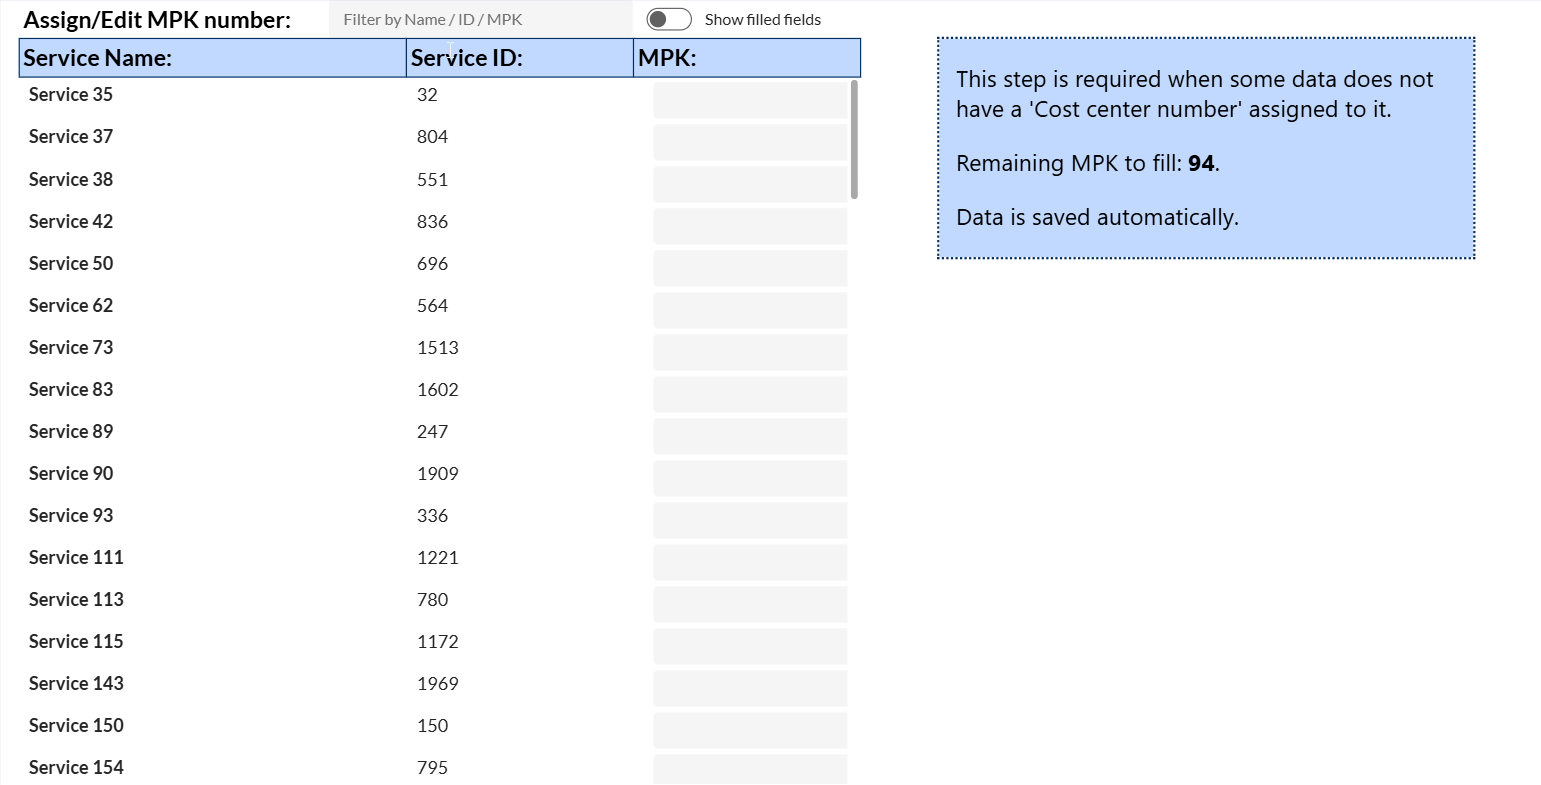
\includegraphics[width=\textwidth]{figures/FillMPKForm.png}
%     \caption{Formularz wypełniania/edycji numerów MPK}
%     \label{fig:fillmpkform}
% \end{figure}
\section{Ekran startowy aplikacji i przygotowanie danych}
\label{relacje-list}
\sectionauthor{R. Wolniak}

Kiedy dane zostały dostosowane do działania systemu, przystąpiono do implementacji pozostałych części rozwiązania.
Kolejnym elementem jest ekran startowy aplikacji, zawierający przyciski, które przekierowują użytkownika do odpowiednich sekcji aplikacji.



Dodatkowo, podczas uruchomienia aplikacji, pobierane są dane z list SharePoint a następnie odpowiednio przetwarzane w celu płynnego wyświetlania ich w aplikacji. \\
Kod w języku \emph{Power Fx} wywoływany podczas uruchamiania aplikacji został przedstawiony w listingu \ref{lst:OnStartCode}.

\lstset{language=C,caption={Kod wywoływany podczas uruchamiania aplikacji},label=lst:OnStartCode}
\begin{lstlisting}[language=PowerFx]
    // Ustawienie zmiennej varDownloadingData na true, aby wskazać, że trwa proces pobierania danych
Set(varDownloadingData, true);

// Tworzenie kolekcji colYears, która zawiera pięć lat: dwa lata wstecz, bieżący rok oraz dwa lata do przodu
ClearCollect(colYears,
    {Value: Text(Now(), "yyyy") - 2},
    {Value: Text(Now(), "yyyy") - 1},
    {Value: Text(Now(), "yyyy") + 0},
    {Value: Text(Now(), "yyyy") + 1},
    {Value: Text(Now(), "yyyy") + 2}
);

// Ustawienie zmiennej VWBlue na kolor o wartości heksadecymalnej #002e5f
Set(VWBlue, ColorValue("#002e5f"));

// Tworzenie kolekcji colNumbers, która zawiera liczby od 1 do 5
ClearCollect(colNumbers,
    {Value: 1}, {Value: 2}, {Value: 3}, {Value: 4}, {Value: 5}
);

// Pobranie profilu użytkownika z usługi Office 365 i przypisanie go do zmiennej UserVar
Set(UserVar, UżytkownicyusługiOffice365.MyProfile());

// 1. Pobieranie danych z Lista_Uslug w partiach
Clear(LocalServiceData); // Wyczyszczenie kolekcji LocalServiceData przed rozpoczęciem pobierania
ForAll(Sequence(Round((First(Sort(Lista_Uslug, 'Identyfikator (ID)', SortOrder.Descending)).'Identyfikator (ID)' - First(Sort(Lista_Uslug, 'Identyfikator (ID)', SortOrder.Ascending)).'Identyfikator (ID)') / 2000 + 1, 0), 1, 1),
    With({
        _firstID: First(Sort(Lista_Uslug, 'Identyfikator (ID)', SortOrder.Ascending)).'Identyfikator (ID)' + (ThisRecord.Value - 1) * 2000,
        _lastID: First(Sort(Lista_Uslug, 'Identyfikator (ID)', SortOrder.Ascending)).'Identyfikator (ID)' + ThisRecord.Value * 2000
    },
    Collect(LocalServiceData, Filter(Lista_Uslug, 'Identyfikator (ID)' >= _firstID && 'Identyfikator (ID)' < _lastID)))
);

// 2. Pobieranie danych z Lista_Kwot w partiach
Clear(LocalCostData); // Wyczyszczenie kolekcji LocalCostData przed rozpoczęciem pobierania
ForAll(Sequence(Round((First(Sort(Lista_Kwot, ID, SortOrder.Descending)).ID - First(Sort(Lista_Kwot, ID, SortOrder.Ascending)).ID) / 2000 + 1, 0), 1, 1),
    With({
        _firstID: First(Sort(Lista_Kwot, ID, SortOrder.Ascending)).ID + (ThisRecord.Value - 1) * 2000,
        _lastID: First(Sort(Lista_Kwot, ID, SortOrder.Ascending)).ID + ThisRecord.Value * 2000
    },
    Collect(LocalCostData, Filter(Lista_Kwot, ID >= _firstID && ID < _lastID)))
);

// 3. Pobieranie danych z Lista_Indykacji w partiach
Clear(LocalIndicationsData); // Wyczyszczenie kolekcji LocalIndicationsData przed rozpoczęciem pobierania
ForAll(Sequence(Round((First(Sort(Lista_Indykacji, ID, SortOrder.Descending)).ID - First(Sort(Lista_Indykacji, ID, SortOrder.Ascending)).ID) / 2000 + 1, 0), 1, 1),
    With({
        _firstID: First(Sort(Lista_Indykacji, ID, SortOrder.Ascending)).ID + (ThisRecord.Value - 1) * 2000,
        _lastID: First(Sort(Lista_Indykacji, ID, SortOrder.Ascending)).ID + ThisRecord.Value * 2000
    },
    Collect(LocalIndicationsData, Filter(Lista_Indykacji, ID >= _firstID && ID < _lastID)))
);

// 4. Łączenie danych z Lista_Uslug, Lista_Kwot i Lista_Indykacji
ClearCollect(MergedData,
    AddColumns(LocalServiceData As ServiceRecord,
        Kwoty,
        With({
            MaxYearCostRecord: First(Sort(Filter(LocalCostData, Service_ID = ServiceRecord.Service_ID), Year, SortOrder.Descending))
        },
        If(IsBlank(MaxYearCostRecord), Blank(), LookUp(LocalCostData, Service_ID = ServiceRecord.Service_ID && Year = MaxYearCostRecord.Year))),
        Indykacje,
        With({
            MaxYearRecord: First(Sort(Filter(LocalIndicationsData, Service_ID = ServiceRecord.Service_ID), Year, SortOrder.Descending))
        },
        If(IsBlank(MaxYearRecord), Blank(), LookUp(LocalIndicationsData, Service_ID = ServiceRecord.Service_ID && Year = MaxYearRecord.Year && IndicationNo = MaxYearRecord.IndicationNo)))
    )
);

// Ustawienie zmiennej varDownloadingData na false, aby wskazać, że proces pobierania danych został zakończony
Set(varDownloadingData, false);
\end{lstlisting}

W pierwszym kroku, zmiennej \emph{varDownloadingData} przypisywana jest wartość \emph{true} za pomocą funkcji \emph{Set()}. Zmienna ta pełni kluczową rolę w zarządzaniu interfejsem użytkownika podczas procesu ładowania danych – aktywuje wskaźnik ładowania oraz blokuje możliwość wprowadzania zmian przez użytkownika, co zapobiega ewentualnym błędom wynikającym z prób modyfikacji danych w trakcie ich pobierania.

Następnie, funkcja \emph{ClearCollect()} tworzy kolekcję \emph{colYears}, która zawiera pięć elementów reprezentujących zakres lat: od dwóch lat wstecz do dwóch lat naprzód. Analogicznie, tworzona jest kolekcja \emph{colNumbers}, zawierająca numery indykacji, które mogą być wykorzystywane w polach typu \emph{Dropdown}. Kolekcje te są niezbędne do budowy dynamicznego i responsywnego interfejsu użytkownika, umożliwiając łatwe zarządzanie danymi w aplikacji.

W kolejnym kroku, za pomocą funkcji \emph{Set()}, pobierane są informacje o aktualnie zalogowanym użytkowniku i przypisywane do zmiennej \emph{UserVar}. Informacje te mogą być wykorzystywane do personalizacji interfejsu użytkownika lub kontroli dostępu do poszczególnych funkcji aplikacji, w zależności od uprawnień użytkownika.

Aplikacja tworzy lokalne kopie trzech list danych: \emph{Lista_Usług}, \emph{Lista_Kwot} oraz \emph{Lista_Indykacji}, wykorzystując funkcję \emph{ClearCollect()}. Dane są pobierane w partiach po 2000 rekordów, aby zoptymalizować wydajność i uniknąć przekroczenia limitów pamięciowych. Proces ten polega na iteracyjnym przetwarzaniu danych, gdzie dla każdej listy określany jest zakres identyfikatorów (ID) pochodzących z listy Sharepoint dla kolejnych partii, zaczynając od najmniejszego ID i zwiększając go o 2000. Każda partia jest filtrowana według tego zakresu i dodawana do odpowiedniej kolekcji lokalnej. Takie podejście pozwala na szybsze przetwarzanie danych i uniknięcie problemów przy pobieraniu dużych zestawów danych.

Kolejnym krokiem jest utworzenie kolekcji \emph{MergedData}, która łączy dane z trzech lokalnych kopii list. W tym celu zastosowano funkcję \emph{AddColumns()}, aby dodać dwie nowe kolumny: \emph{Kwoty} oraz \emph{Indykacje}. Funkcja \emph{With()} pozwala na uproszczenie złożonych obliczeń poprzez przypisanie wyników pośrednich do zmiennych, co zwiększa czytelność kodu. Dane w kolumnach są wyodrębniane przy użyciu funkcji \emph{LookUp()} oraz \emph{Filter()}, które umożliwiają precyzyjne filtrowanie i wyszukiwanie rekordów na podstawie trzech kluczowych kryteriów: \emph{Service_ID}, \emph{Year} oraz \emph{IndicationNo}.

W efekcie, kolekcja \emph{MergedData} zawiera dane dla najnowszego roku i najwyższego numeru indykacji dla każdej usługi, co umożliwia prezentację aktualnych informacji w interfejsie użytkownika.

Na końcu procesu, zmiennej \emph{varDownloadingData} przypisywana jest wartość \emph{false}, co sygnalizuje zakończenie pobierania danych i gotowość aplikacji do użytku. Lokalne kopie list (\emph{LocalServiceData}, \emph{LocalCostData}, \emph{LocalIndicationsData}) zostały utworzone w celu przyspieszenia działania mechanizmu filtrowania oraz zwiększenia efektywności podczas wyboru usług do edycji.





\section{Edycja danych}
\sectionauthor{M. Gajdzis}

Po zapisaniu najnowszych danych kolejnym krokiem jest wprowadzenie niezbędnych aktualizacji dotyczących usług. W tym celu zaimplementowano dwa ekrany: pierwszy służący do wyboru usługi z listy oraz drugi, który umożliwia przeglądanie i edycję szczegółów związanych z wybraną usługą. Oba ekrany zostały zaprojektowane z myślą o intuicyjnej nawigacji i efektywnym zarządzaniu danymi.

\subsection{Ekran wyboru usługi do edycji}

% \begin{figure}[h]
% \centering
% 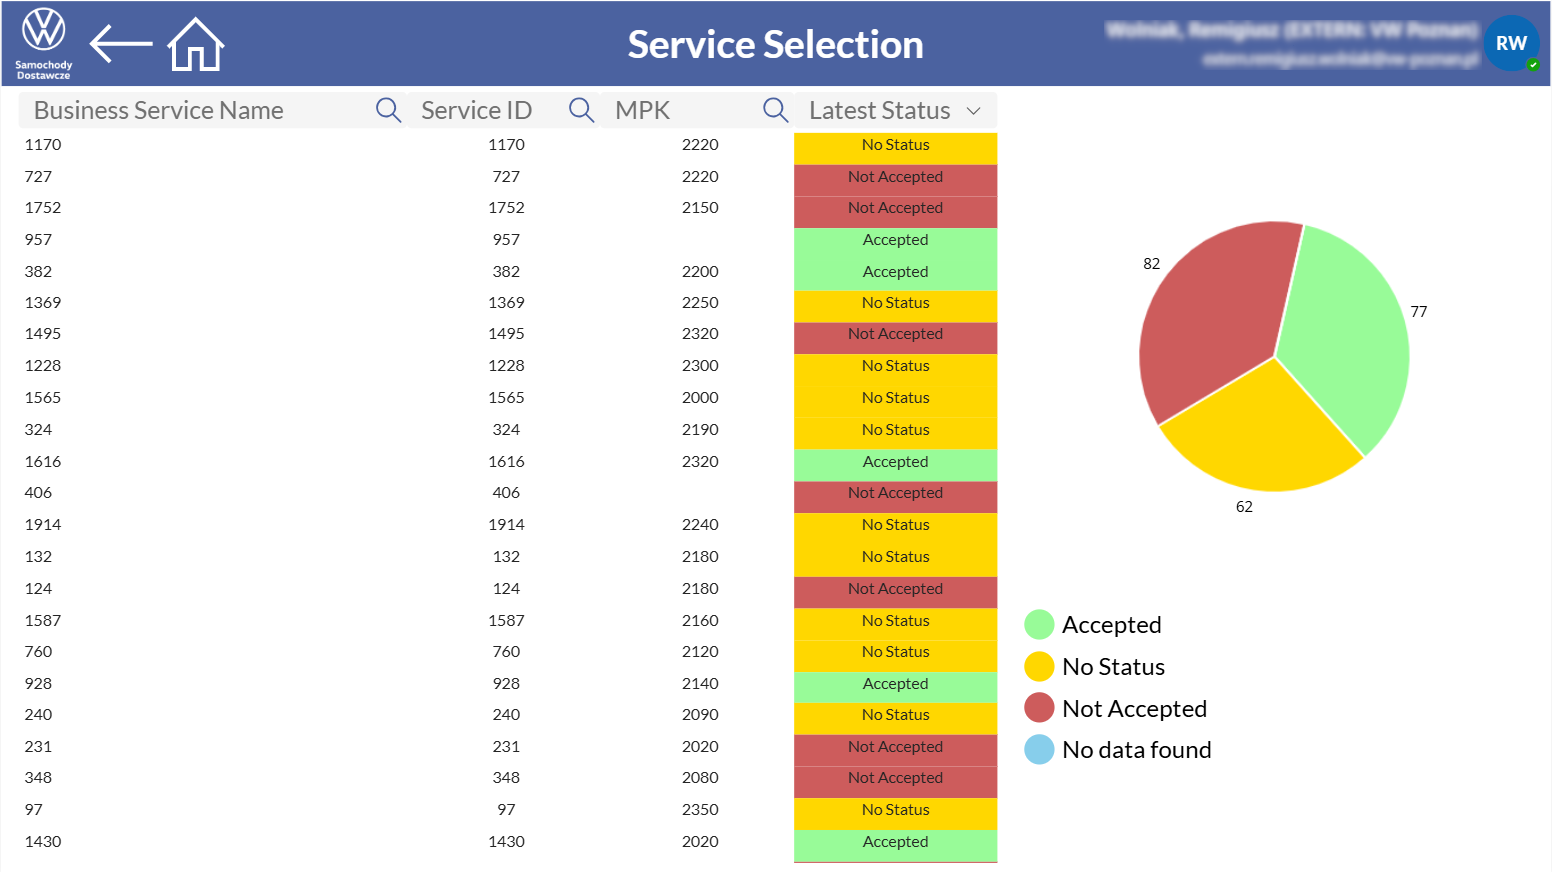
\includegraphics[width=0.9\textwidth]{figures/ServiceSelectionForm.png}
% \caption{Ekran wyboru usługi do edycji}
% \label{fig:ServiceSelectionForm }
% \end{figure}

Ekran wyboru usługi do edycji został zaprojektowany w sposób umożliwiający użytkownikom szybkie i precyzyjne wyszukiwanie oraz filtrowanie danych. Składa się z następujących elementów:

\subsubsection*{Lista wyboru serwisu}

Lista prezentuje dane pochodzące z dynamicznej kolekcji \emph{MergedData}, która została szczegółowo omówiona w poprzednim podrozdziale. Dzięki temu użytkownicy mają dostęp do aktualnych informacji bez konieczności ręcznego przeszukiwania list źródłowych.

Każdy element na liście posiada dodatkową funkcję interakcji. Po najechaniu kursorem na wybraną usługę (właściwość \emph{Hover}), element wizualnie zmienia swój wygląd -- zwęża się oraz zmienia kolor. Kliknięcie wybranego elementu przenosi użytkownika do dedykowanego ekranu edycji, który umożliwia szczegółowe zarządzanie wybraną usługą.

Dodatkowo użytkownik ma możliwość zawężenia widocznych danych poprzez zastosowanie różnych kryteriów wyszukiwania. Pola obejmują:

\begin{itemize}
    \item \textbf{Wyszukiwanie po nazwie usługi (\emph{Service Name})} -- Obsługuje częściowe dopasowania dzięki wbudowanej funkcji \emph{StartsWith}, która sprawdza, czy ciąg tekstowy zaczyna się od określonej frazy.
    \item \textbf{Filtrowanie po identyfikatorze usługi (\emph{Service ID})} -- Umożliwia precyzyjne wyszukiwanie konkretnego elementu względem jego identyfikatora (\emph{Service ID}).
    \item \textbf{Filtrowanie według miejsca powstawania kosztów (\emph{MPK})} -- Pozwala na szybkie odnalezienie danych przypisanych do konkretnego obszaru finansowego.
    \item \textbf{Filtrowanie według statusu decyzji (\emph{Accepted}, \emph{Not Accepted}, \emph{No Status})}.
\end{itemize}

Filtry te mogą być stosowane jednocześnie, co umożliwia dokładne dopasowanie wyświetlanych danych.

Warto zauważyć, że informacje dotyczące podjętej decyzji są przechowywane w bazie danych w postaci liczb całkowitych w celu szybszego przeszukiwania. Aby jednak w aplikacji widoczne były one w postaci tekstowej, zastosowano funkcję \emph{Switch}, która przypisuje odpowiednią wartość tekstową na podstawie wartości liczbowej.

\subsubsection*{Wykres kołowy}
\par
Ostatnim elementem tego ekranu jest wykres kołowy, który ilustruje podział danych według statusów decyzji.
Dane widoczne na wykresie pochodzą z listy wyboru usługi, co pozwala na uwzględnienie filtrów, np. po wprowadzeniu numeru MPK użytkownik może sprawdzić jaka część usług należąca do danego obszaru wymaga rozpatrzenia. Wartości przekazane są do właściwości \emph{Items} i uwzględniają mapowanie wartości liczbowych na tekst.



\subsection{Ekran edycji elementu}

Ekran edycji elementu prezentuje szczegółowe informacje dotyczące wybranej usługi, umożliwiając analizę danych historycznych oraz wprowadzanie nowych decyzji. Ekran składa się z kilku logicznie ułożonych sekcji, które są opisane poniżej.


\subsubsection*{Porównanie finalnych decyzji z lat poprzednich}

W górnej części ekranu umieszczona została galeria, przedstawiająca porównanie danych finansowych oraz decyzji z trzech ostatnich lat. Dane, określone we właściwości \emph{Items}, zawierają:

\begin{itemize}
    \item \textbf{Rok (Year)} -- okres, którego dotyczy dana decyzja.
    \item \textbf{Jednostka miary (Unit Of Measurement)} -- zazwyczaj ilość licencji.
    \item \textbf{Zeszłoroczne i planowane na następny rok wartości finansowe} -- \emph{Current Year Plan} oraz \emph{Next Year Plan}.
    \item \textbf{Różnice w finansach (Difference)} -- różnica między zeszłorocznymi i potencjalnymi przyszłymi kosztami.
    \item \textbf{Status końcowej decyzji (Final Decision)} -- decyzje dotyczące finalnej decyzji z danego roku (\emph{Accepted, Not Accepted, No Status}).
\end{itemize}


% \subsubsection*{Link do instrukcji obsługi}

% Poniżej tabeli z porównaniem decyzji znajduje się link do dedykowanej instrukcji obsługi usługi. Za pomocą linku użytkownik posiada dostęp do szczegółowych informacji na temat zasad korzystania z danej usługi, co może być przydatne podczas edycji danych lub wprowadzania nowych decyzji.

Galeria ta jest interaktywna. Oznacza to, że po kliknięciu na wybrany wiersz, wyświetlana jest kolejna galeria, która zawiera szczegółowe informacje na temat poszczególnych indykacji z wybranego roku.

\subsubsection*{Porównanie tegorocznych indykacji}

Druga galeria wyświetla następujące informacje:
\begin{itemize}
    \item \textbf{Numer indykacji (Indication Number)},
    \item \textbf{Komentarze} -- w tym \emph{Internal Comment, Comment PZ to WOB, Comment K-DES},
    \item \textbf{Data i autor komentarza},
    \item \textbf{Status decyzji (Decision)}.
\end{itemize}

Aby uniknąć problemu z czytelnością długich komentarzy, które nie mieszczą się w przeznaczonych komórkach, zaimplementowano możliwość kliknięcia na element. Skutkuje to ustawieniem wartości zmiennej \emph{ShowCommentPopup}, odpowiedzialnej za widoczność okna dialogowego, na wartość \emph{True}. W oknie tym wyświetlany jest autor, data wprowadzenia oraz pełna treść komentarza. Dane dotyczące komentarza przekazywane są w zmiennej tablicowej \emph{SelectedComment}, która aktualizowana jest w momencie wybrania komórki z komentarzem.

\subsubsection*{Formularz do uzupełnienia danych}

Na samym dole strony znajduje się formularz umożliwiający wprowadzenie nowych danych lub aktualizację istniejących rekordów. Formularz zawiera pola takie jak:
\begin{itemize}
    \item \textbf{Rok (\emph{Year})} -- pole typu \emph{Dropdown}, zawiera dane z kolekcji \emph{colYears} tworzonej przy uruchomieniu aplikacji,
    \item \textbf{Numer indykacji (\emph{Indication Number})} -- pole typu \emph{Dropdown}, zawiera dane z kolekcji \emph{colNumbers} tworzonej przy uruchomieniu aplikacji,
    \item \textbf{Komentarze} -- pole \emph{TextInput} (wprowadzania tekstu),
    \item \textbf{Status decyzji (\emph{Decision})} -- pole typu \emph{Dropdown}. Dane we właściwości \emph{Items}, zdefiniowane są jako \emph{["Accepted", "No Status", "Not Accepted"]}.
    \item \textbf{Data} -- kontrolka \emph{DatePicker}, która umożliwia wybór daty poprzez wyświetlenia kalendarza,
    \item \textbf{Autor} -- pole \emph{ComboBox}, umożliwia wybór autora z listy pracowników. Lista ta pobierana jest poprzez connector \emph{Office365Users}\footnote{\emph{Office365Users} -- konektor pozwalający na dostęp do listy zawierającej informacje na temat użytkowników takie jak imię, nazwisko, dane kontaktowe lub dział.}, który zawiera informacje na temat wszystkich użytkowników infrastruktury firmy.
\end{itemize}


\subsubsection*{Przycisk zapisu}


Ostatnim elementem na tym ekranie jest przycisk \emph{Save}, który umożliwia zapisanie wprowadzonych zmian. Mechanizm ten:

\begin{itemize}
    \item Sprawdza istnienie wcześniejszych indykacji, aby upewnić się, że zachowana jest poprawna kolejność numeracji.
    \item W przypadku istniejącego wpisu -- uzupełnia dane przy użyciu funkcji \emph{Patch}.
    \item W przypadku nowego wpisu -- tworzy nowy rekord przy użyciu funkcji \emph{Defaults}.
    \item Resetuje pola formularza oraz odświeża dane na ekranie, aby uwzględnić ostatnie zmiany.
    \item Informuje użytkownika o powodzeniu lub błędach operacji za pomocą komunikatów (\emph{Notify}).
\end{itemize}

\subsection{Listing kodu}

Listing \ref{lst:SaveFormCode} przedstawia fragment kodu odpowiedzialny za zapisywanie danych w formularzu edycji, który jest wywoływany po kliknięciu przycisku \emph{Save}. Kod ten odpowiedzialny jest za zapisanie informacji z formularza w bazie danych.

\begin{lstlisting}[language=PowerFx, caption={Kod zapisywania danych w formularzu edycji}, label=lst:SaveFormCode ]
    If(
        // Dla indykacji nr 1
        IndicationNo_Dropdown.Selected.Value = 1;
        
        // Sprawdź; czy istnieje już pierwsza indykacja
        If(
            !IsBlank(
                LookUp(
                    Lista_Indykacji;
                    Year = Year_Dropdown.Selected.Value &&
                    IndicationNo = 1 &&
                    Service_ID = ChosenServiceID
                )
            );
            // Aktualizacja istniejącego rekordu
            Set(
                TempOutput;
                Patch(
                    Lista_Indykacji;
                    LookUp(
                        Lista_Indykacji;
                        Year = Year_Dropdown.Selected.Value &&
                        IndicationNo = 1 &&
                        Service_ID = ChosenServiceID
                    );
                    {
                        Comment_date: Text(CommentDateInput.SelectedDate);
                        Comment_author: ComboboxCanvas1.Selected.DisplayName;
                        Comment_PZ_to_WOB: CommentToWOBInput.Value;
                        Comment_Intern: InternalCommentInput.Value;
                        Decision: Switch(
                            DropdownCanvas1.Selected.Value;
                            "Accepted"; 1;
                            "No Status"; 0;
                            "Not Accepted"; -1;
                            0
                        )
                    }
                )
            );;
            Notify("A record has been successfully updated!"; NotificationType.Success);
            
            // Jeśli rekord nie istnieje; utwórz nowy
            Set(
                TempOutput;
                Patch(
                    Lista_Indykacji;
                    Defaults(Lista_Indykacji);
                    {
                        Service_ID: ChosenServiceID;
                        Year: Year_Dropdown.Selected.Value;
                        IndicationNo: 1;
                        Comment_date: Text(CommentDateInput.SelectedDate);
                        Comment_author: ComboboxCanvas1.Selected.DisplayName;
                        Comment_PZ_to_WOB: CommentToWOBInput.Value;
                        Comment_Intern: InternalCommentInput.Value;
                        Decision: Switch(
                            DropdownCanvas1.Selected.Value;
                            "Accepted"; 1;
                            "No Status"; 0;
                            "Not Accepted"; -1;
                            0
                        )
                    }
                )
            );;
            Notify("The record has been successfully created!"; NotificationType.Success)
        )
    );;    
\end{lstlisting}
\section{Generowanie raportu}
\sectionauthor{M. Gajdzis}

Następnym ekran umożliwia wygenerowania raportu w formacie arkusza kalkulacyjnego na podstawie uzupełnionej bazy danych. W związku z tym w Power Apps przygotowano mechanizm łączący dane z trzech list SharePoint, które następnie są przesyłane do Power Automate, gdzie podlegają dalszemu przetwarzaniu. Wynikiem tego jest kompletny arkusz Excel, który jest zapisywany na platformie SharePoint.

\subsection{Łączenie danych z list}

W celu określenia, roku i indykacji których ma dotyczyć raport, wprowadzono kontrolki \emph{Dropdown} po lewej stronie ekranu. Ich uzupełnienie skutkuje wygenerowaniem podglądu danych, który pozwala na walidację ich poprawności. Listing \ref{lst:combineddata} przedstawia kod odpowiedzialny za utworzenie kolekcji \emph{CombinedData}, która zawiera odpowiednio odfiltrowane informacje.


% Zebrane dane przechowywane są w tymczasowej kolekcji \emph{CombinedData}, która składa się z informacji z trzech źródeł, odpowiednio dopasowanych do wybranego przez użytkownika roku oraz indykacji. Przykładowy fragment kodu odpowiedzialnego za tworzenie tej kolekcji przedstawiono w listingu~\ref{lst:combineddata}:

\begin{lstlisting}[language=PowerFx, caption={Fragment kodu tworzącego kolekcję CombinedData}, label={lst:combineddata}] 
    ClearCollect(
    CombinedData;
    AddColumns(
        LocalServiceData;
        MPK;
        LookUp(
            LocalCostData;
            Service_ID = LocalServiceData[@Service_ID] && Year = Year_Dropdown_1.Selected.Value;
            MPK
        );
        Comment_PZ_to_WOB;
        LookUp(
            LocalIndicationsData;
            Service_ID = LocalServiceData[@Service_ID] && Year = Year_Dropdown_1.Selected.Value && IndicationNo = IndicationNo_Dropdown_1.Selected.Value;
            Comment_PZ_to_WOB);     
    [...]
);;

\end{lstlisting}

Kod ten korzysta z następujących funkcji:
\begin{itemize}
    \item \emph{ClearCollect} -- przypisuje dane do kolekcji o podanej nazwie,
    \item \emph{AddColumns} -- pozwala na dodanie do kolekcji nowej kolumny i formuły definiującej jej wartości,
    \item \emph{LookUp} -- wyszukuje rekordy w tabeli na podstawie podanych kryteriów.
\end{itemize}

\subsection{Przekazywanie danych do Power Automate}

W lewym dolnym rogu interfejsu znajduje się przycisk \emph{Generate file}, który po naciśnięciu uruchamia przepływ Power Automate, odpowiedzialny za stworzenie pliku na podstawie danych wejściowych. Dane te są przekazywane do usługi Power Automate w postaci ciągu tekstowego, sformatowanego jako JSON\footnote{JSON - format wymiany danych, który jest oparty na strukturze tekstowej}, wykorzystując połączone informacje z trzech źródeł zawarte w kolekcji \emph{CombinedData}. Kod wywołujący funkcję \emph{GenerateRaport} przedstawiono w listingu~\ref{lst:generateraport}.



\begin{lstlisting}[language=PowerFx, caption={Kod wywołujący funkcję GenerateRaport}, label={lst:generateraport}]
    GenerateRaport.Run(
        Substitute(
            "[" & 
            Concat(
                CombinedData;
                "{""Service_ID"":""" & Service_ID & """," &
                """Service_Name"":""" & Service_Name & """," &
                """MPK"":""" & MPK & """," &
                """Comment_PZ_to_WOB"":""" & Comment_PZ_to_WOB & """," &
                """Decision"":""" & Decision & """},"
            ) & 
            "]",
            "},]"; 
            "}]"
        ),
        IndicationNoCollect.Value,
        YearNoCollect.Value
    )
    \end{lstlisting}



\subsection{Generowanie raportu w Power Automate}


\emph{Flow} o nazwie \emph{GenerateRaport} składa się z kilku komponentów, które 
pozwalają na stworzenie raportu w formacie arkusza kalkulacyjnego, w oparciu o dane z list SharePoint. Przepływ ten zawiera następujące instrukcje:

\begin{itemize}
    \item \textbf{Wejście danych:} \emph{Flow} przyjmuje trzy dane wejściowe: ciąg znaków w formacie JSON, zawierający dane przekazane z aplikacji do przetworzenia, wybraną indykację oraz wybrany rok.
    \item \textbf{Inicjalizacja zmiennej:} W tym kroku tworzona jest zmienna odpowiedzialna za nazwę generowanego pliku. Zmienna zawiera dynamicznie generowaną datę utworzenia pliku.
    \item \textbf{Generowanie pustego arkusza Excel:} Wykorzystywany jest statyczny plik Excel, zapisany w formacie Base64, który pełni rolę szablonu dla dalszego przetwarzania.
    \item \textbf{Tworzenie pliku na SharePoint:} Szablon arkusza zostaje zapisany w określonej lokalizacji w bibliotece SharePoint.
    \item \textbf{Sprawdzenie dostępności pliku:} W celu upewnienia się, że plik jest gotowy do dalszego przetwarzania, uruchamiana jest pętla \emph{Do until}, która weryfikuje dostępność pliku na platformie.
    \item \textbf{Uruchomienie skryptu:} Na końcu przepływu wywoływany jest skrypt pakietu office, który generuje wypełniony arkusz Excel.
\end{itemize}

Schemat \ref{fig:generateflowcomponent} przedstawia szczegółowy schemat przepływu, uwzględniający poszczególne kroki oraz przepływ danych między nimi.

\begin{figure}[H]
    \centering
    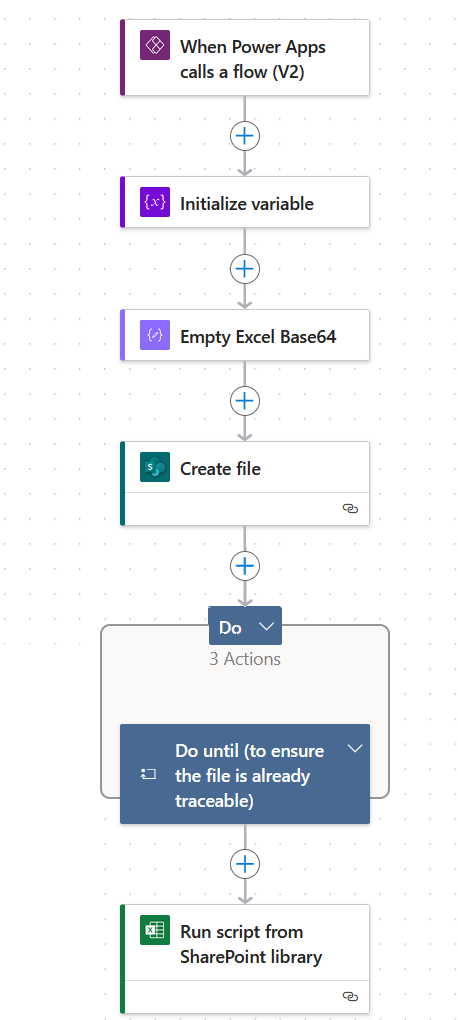
\includegraphics[width=0.45\textwidth]{figures/GenerateRaportFlow.png}
    \caption{Schemat przepływu \emph{GenerateRaport}}
    \label{fig:generateflowcomponent}
\end{figure}

\subsubsection*{Opis działania skryptu generującego raport}

Skrypt odpowiedzialny za generowanie raportu wykonuje kilka operacji. Jego główne funkcje to:
\begin{itemize}
    \item \textbf{Analiza danych wejściowych:} Przyjęcie danych w formacie JSON oraz roku. W przypadku otrzymania niepoprawnych dancyh, w arkuszu umieszczony jest odpowiedni komunikat.
    \item \textbf{Tworzenie arkusza:} Sprawdzenie, czy arkusz wynikowy już istnieje -- jeśli tak, to usuwa go i tworzy nowy.
    \item \textbf{Dynamiczne wstawianie danych:} Kolumny zawierające informacje na temat cen, mają w nagłówkach podany rok, których one dotyczą.
    \item \textbf{Generowanie tabeli:} Tworzenie nagłówków tabel (np. \texttt{Service\_ID}, \texttt{Service\_Name}) oraz wprowadzenie danych wypełniające tabelę, pobierane z JSON.
    \item \textbf{Formatowanie:} Skrypt aktywuje opcję filtracji kolumn oraz zmienia ich szerokość. Dzięki temu arkusz jest czytelny i nie wymaga formatowania ze strony użytkownika.
\end{itemize}






\begin{comment}
W niniejszym rozdziale przedstawiono szczegóły techniczne zaimplementowanego rozwiązania. Omówione zostaną kluczowe aspekty
implementacyjne systemu, obejmujące wykorzystanie platformy Microsoft Power Platform - w szczególności
Power Apps do budowy interfejsu użytkownika oraz Power Automate do automatyzacji procesów biznesowych.
Ponadto, przedstawiona zostanie integracja z platformą SharePoint oraz implementacja skryptów
usprawniających pracę z pakietem Microsoft Office. Rozdział stanowi techniczne rozwinięcie przyjętych
założeń projektowych, prezentując metodykę realizacji poszczególnych komponentów systemu.

W ramach analizy technicznej zostaną szczegółowo omówione poszczególne komponenty systemu oraz sposób
ich integracji. Szczególna uwaga zostanie poświęcona mechanizmom przepływu danych, automatyzacji
procesów oraz implementacji logiki biznesowej w środowisku low-code. Ponadto poruszono napotkane problemy oraz ich rozwiązania.

\section{Ekran zapisu danych}

Zdecydowano, że pierwszym ekranem aplikacji będzie ekran zapisu danych. Decyzja ta wynika z faktu, że bez prztworzonych danych, utworzenie innych ekranów byłoby zdecydowanie trudniejsze. Ekran ten składa się z elementów, które zostaną omówione poniżej.

\subsection{Zapis pliku w chmurze}
Pierwszym krokiem jest zapis pliku w chmurze w celu udostepnienia go innym systemom. W tym celu wykorzystano kontrolkę\footnote{Kontrolka -- element służący do nawigacji, wyświetlania danych i obsługi aplikacji.} \emph{Attachment Control}. Pozwala ona na zapisanie pliku w pamięci aplikacji. Odbywa się to przez naciśnięcie przycisku \emph{"Dołącz plik"} lub przy użyciu mechaniki \emph{przeciągnij i upuść} (\english{Drag And Drop}). 

Aby przekazać plik oraz jego zawartość należy nacisnąć przycisk opisany jako \emph{Save attachments} znajdujący się pod wcześniej omawianym elementem. Naciścięcie go skutkuje wywołaniem szeregu funkcji opisanych we właściwości \emph{OnSelect}. W pierwszej kolejności sprawdzane jest, czy plik został załadowany. Jeśli tak, to wywoływany jest przepływ \emph{SaveFileAndRunScript}. Wynik przepływu jest zapisywany w zmiennej tablicowej, która w Power Apps określana jest jako \definicja{kolekcja}, o nazwie \emph{FlowOutput}. Po wykonaniu się przepływu, zapisane w kontrolce pliki są usuwane.

\subsubsection{Przepływ SaveFileAndRunScript}
Przepływ \emph{SaveFileAndRunScript} jest odpowiedzialny za zapisanie pliku w chmurze. W momencie wywołania przepływu plik jest przekazany jako parametr wejściowy. Przepływ ten składa się z kilku kroków, które zostaną omówione w kolejności ich wykonywania.

\begin{figure}[H]
    \centering
    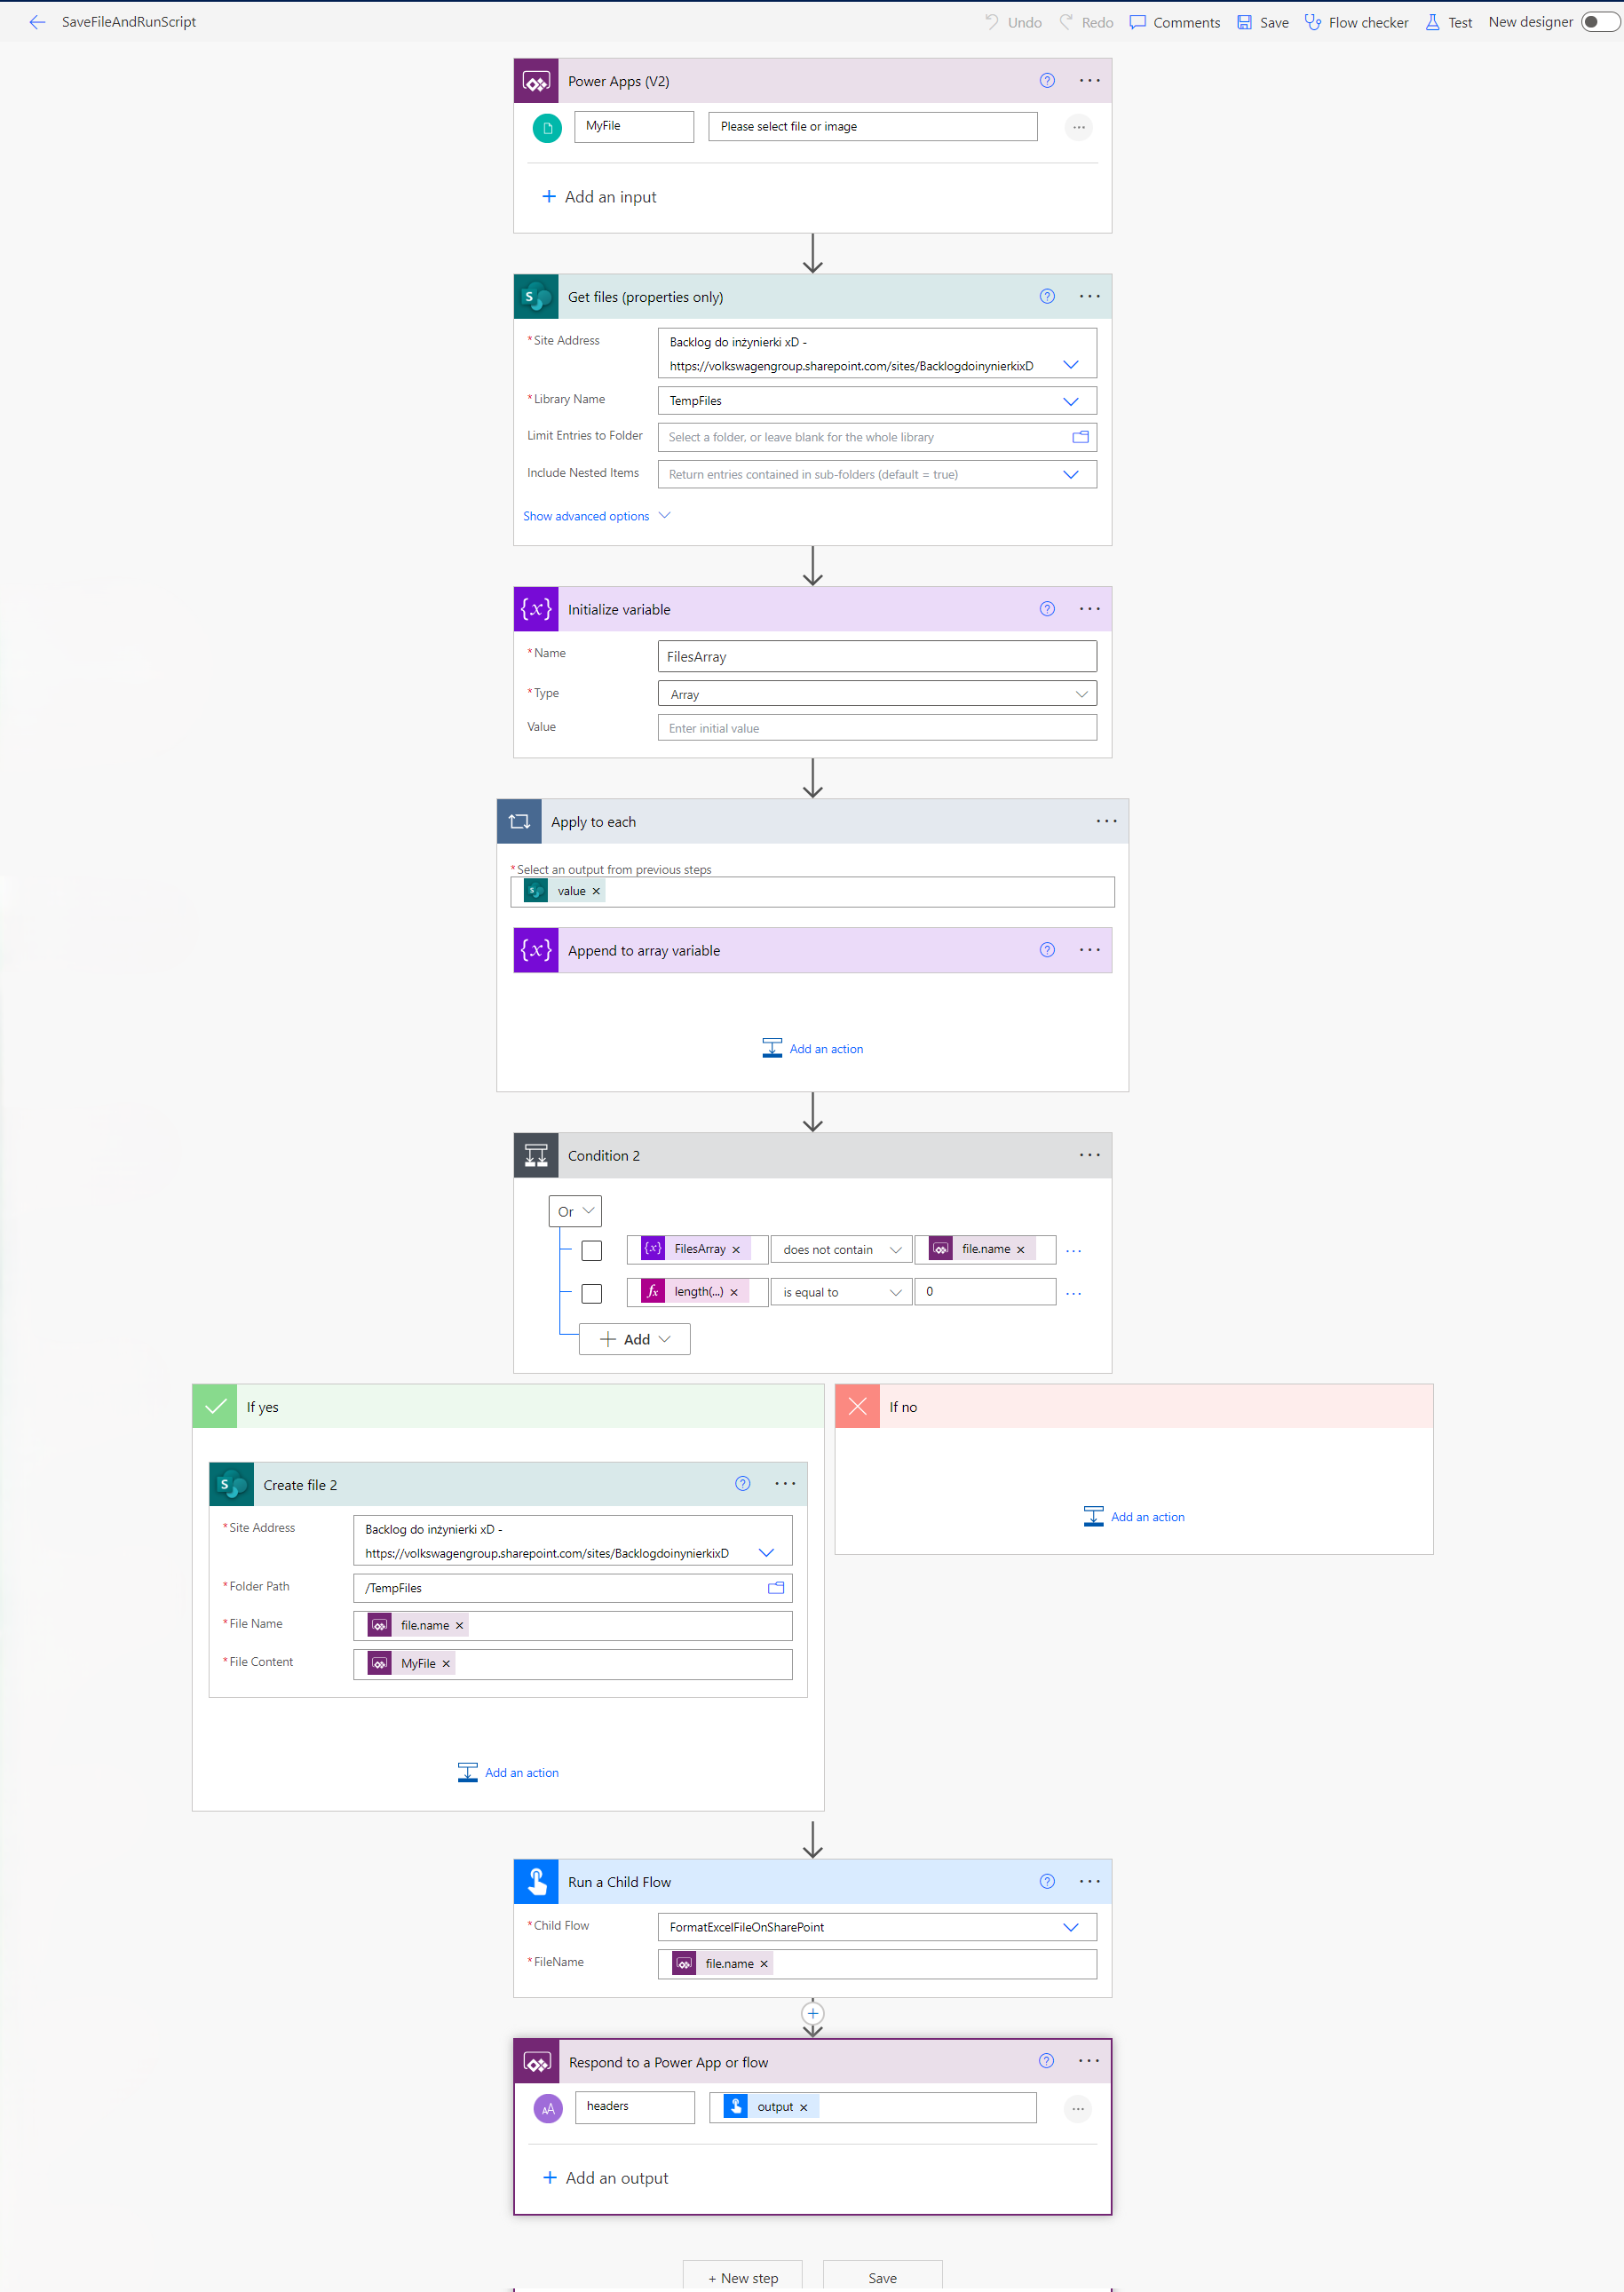
\includegraphics[width=0.85\textwidth]{figures/SaveFileAndRunScript.png}
    \caption{Widok przepływu SaveFileAndRunScript}
    \label{fig:savefileandrunscript}
\end{figure}

Rysunek \ref{fig:savefileandrunscript}, przedstawia widok przepływu \emph{SaveFileAndRunScript}. Przepływ ten składa się z następujących kroków:
\begin{enumerate}
    \item \textbf{Funkcja: Power Apps (V2)} \\
    Jest to element rozpoczynający przepływ, wywoływany bezpośrednio z aplikacji Power Apps. Parametrami wejściowymi są:
    \begin{itemize}
        \item nazwa pliku (\textit{File Name}),
        \item zawartość pliku (\textit{File Content}) w formacie binarnym.
    \end{itemize}

    \item \textbf{Sprawdzenie istniejących plików} \\
    Blok \textit{Get files (properties only)} pobiera listę wszystkich plików z wybranego folderu SharePoint wraz z ich metadanymi, takimi jak nazwa, ścieżka czy data modyfikacji. Pozwala to na sprawdzenie, czy plik o podanej nazwie już istnieje w bibliotece.

    \item \textbf{Warunek} \\
    Element \textit{Condition} sprawdza, czy istnieje plik o nazwie przekazanej w danych wejściowych. W zależności od wyniku:
    \begin{itemize}
        \item jeśli plik istnieje -- przepływ kończy działanie,
        \item jeśli plik nie istnieje -- kontynuuje proces zapisu.
    \end{itemize}

    \item \textbf{Utworzenie pliku} \\
    Blok \textit{Create file} tworzy nowy plik w SharePoint, wykorzystując parametry:
    \begin{itemize}
        \item adres witryny SharePoint,
        \item ścieżkę do folderu docelowego,
        \item nazwę pliku,
        \item zawartość pliku.
    \end{itemize}

    \item \textbf{Uruchomienie podprzepływu} \\
    Element \textit{Run a Child Flow} wywołuje skrypt Office Script, który:
    \begin{itemize}
        \item analizuje zapisany plik,
        \item sprawdza jego zawartość,
        \item formatuje dane według wymagań,
        \item zwraca wynik w formacie JSON.
    \end{itemize}

    \item \textbf{Odpowiedź do aplikacji} \\
    Blok \textit{Respond to Power Apps} kończy przepływ, zwracając do aplikacji dane w formacie JSON przetworzone przez wcześniej wspomniany skrypt Office Script.
\end{enumerate}

\subsection{Skrypt Office Script}
Po utworzeniu pliku w SharePoint, w ramach przepływu następuje jego przetworzenie przez skrypt Office Script. W tym przypadku skrypt ma za zadanie przeanalizować plik i dostosować go do wymagań systemu. Poniżej przedstawiono kroki działania skryptu:

\begin{enumerate}
    \item \textbf{Inicjalizacja i wybór arkusza}
    \begin{itemize}
        \item sprawdzenie wszystkich arkuszy w pliku Excel,
        \item wybór arkusza zawierającego dane,
        \item sprawdzenie i ewentualne usunięcie ochrony hasłem.
    \end{itemize}

    \item \textbf{Analiza danych}
    \begin{itemize}
        \item sprawdzenie czy dane są zorganizowane w tabeli,
        \item w przypadku braku tabeli -- utworzenie nowej,
        \item automatyczne uzupełnienie pustych miejsc w ważnych kolumnach.
    \end{itemize}

    \item \textbf{Dopasowanie nazw kolumn}
    \begin{itemize}
        \item porównanie istniejących nazw kolumn ze standardową listą,
        \item wykorzystanie algorytmu \emph{Jaro-Winkler} do oceny podobieństwa tekstu,
        \item automatyczne rozpoznawanie podobnych nazw (np. "Srv ID" jako "Service ID"),
        \item sugestia ręcznego wyboru przy zbyt małym podobieństwie (poniżej 90\%).
    \end{itemize}

    \item \textbf{Przekazanie wyników}
    \begin{itemize}
        \item zwrócenie oryginalnych nazw kolumn z pliku,
        \item zwrócenie dopasowanych standardowych nazw kolumn,
        \item w razie problemów - przekazanie odpowiednich komunikatów błędów.
    \end{itemize}
\end{enumerate}


\vspace{1cm}
Po zakończeniu działania skryptu Office Script i całego przepływu, przetworzony plik zostaje w pełni zapisany w bibliotece SharePoint. 
Rysunek \ref{fig:saveattachmentsform} przedstawia wspomnianą wcześniej kontrolkę \emph{Attachment Control}, przycisk \emph{Save attachments} oraz listę plików zapisanych w foldrze SharePoint.


\begin{figure}[h]
    \centering
    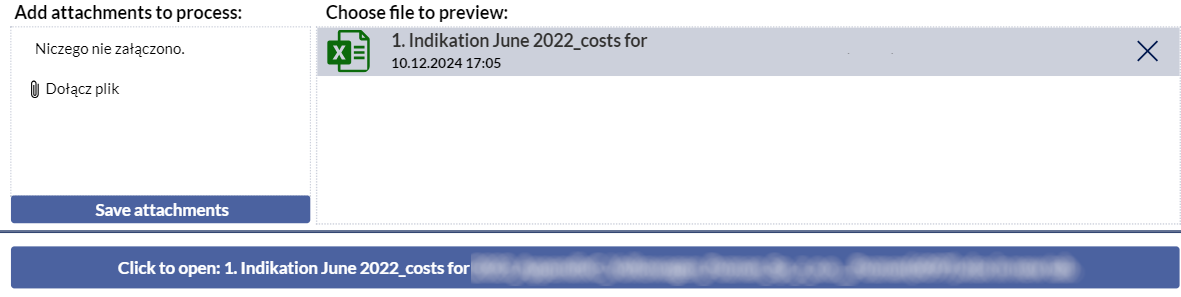
\includegraphics[width=\textwidth]
    {figures/SaveAttachmentsForm.png}
    \caption{Formularz zapisu pliku}    
    \label{fig:saveattachmentsform}
\end{figure}

Wybór elementu z listy \emph{Choose file to preview} umożliwia wskazanie pliku do dalszego przetwarzania. Selekcja pozycji z listy automatycznie inicjuje wykonanie opisanego wcześniej skryptu, którego celem jest pozyskanie aktualnego zestawu nagłówków. Należy podkreślić, że ten sam proces zachodzi również podczas inicjalizacji aplikacji. 
Funkcjonalność podglądu, zaimplementowana w postaci przycisku umiejscowionego poniżej głównych elementów sterujących, umożliwia otwarcie wybranego pliku w nowej karcie przeglądarki. Jest to szczególnie istotne w kontekście weryfikacji poprawności danych oraz walidacji struktury kolumn. \end{comment}